%%%%%%%%%%%%%%%%%%%%%%%%%%%%%%%%%%%%%%
% This is the name of the style file.
%%%%%%%%%%%%%%%%%%%%%%%%%%%%%%%%%%%%%%
%
% phd  -> for a PhD dissertation
% ms   -> for an MS thesis
% If both phd and ms are used then phd will overide.  If none are used,
% then ms will be active by default.
%
% cpyr -> generate a copyright page
% lof  -> generate List of Figures
% lot  -> generate List of Tables
\documentclass[ms,cpyr,lof,lot]{uathesis}

% Subsections in TOC
%% ONLY FOR PLANNING, NOT FOR FINAL COPY %%
\setcounter{tocdepth}{4}
\setcounter{secnumdepth}{4}

%
%%%%%%%%%%%%%%%%%%%%%%%%%%%%%%%%
% List of any packages you use.
%%%%%%%%%%%%%%%%%%%%%%%%%%%%%%%%
%

%% FROM REU SUMMARY


\usepackage{graphicx}
\usepackage{amsmath,amssymb}
%\usepackage{gensymb}
\usepackage{xcolor}
\usepackage{mathtools}
\usepackage{etoolbox}
\usepackage{booktabs}
\usepackage{float}
\usepackage{graphicx}
\usepackage{rotating}
\usepackage{geometry}
\usepackage{multicol}
\usepackage{caption}
\usepackage{natbib}
\usepackage{siunitx}
\usepackage[all]{nowidow}
\usepackage{listings}
\usepackage{layouts}
\usepackage{bm}
\usepackage[outdir=./eps2pdf/]{epstopdf}
\graphicspath{
  {figures/}
  {figures/goals/}
  {figures/light_data/}
  {figures/attenuation/}
  {figures/results/}
}

%%%%%%%%%%%%%%%%%%%%%%%%%%%%%%%%%%
% List of definitions you define.
%%%%%%%%%%%%%%%%%%%%%%%%%%%%%%%%%%

\setlength{\tabcolsep}{12pt}

\definecolor{commentcolor}{HTML}{752000}
\definecolor{keywordcolor}{HTML}{007520}

% Listings
\lstset{
    language=[90]Fortran,
    inputpath=../kelp/code/fortran/src,
    basicstyle=\linespread{0.8}\ttfamily,
    commentstyle=\rmfamily,
    keywordstyle=\color{commentcolor},
    commentstyle=\color{keywordcolor},
    showstringspaces=false,
    numbers=left,
    breaklines=true,
    numbersep=1em,
    frame=leftline,
    tabsize=4,
    xleftmargin=.5in,
    xrightmargin=.5in}

\DeclareMathOperator{\atantwo}{atan2}

% Domain
\newcommand\xmin{{x_{\min}}}
\newcommand\xmax{{x_{\max}}}
\newcommand\ymin{{y_{\min}}}
\newcommand\ymax{{y_{\max}}}
\newcommand\zmin{{z_{\min}}}
\newcommand\zmax{{z_{\max}}}

%% FROM GOALS
\newcommand\plotwidth{7in}

%% FROM REU SUMMARY

\newcommand{\ds}{\displaystyle}

% Define error function for math mode
\newcommand{\erf}{\mbox{erf}}
% Sign function
\newcommand{\sign}{\mbox{sign}}
\newcommand{\ceil}{\mbox{ceil}}
\newcommand{\floor}{\mbox{floor}}
% Real numbers
\newcommand\R{\mathbb{R}}
% Norm
\newcommand\norm[1]{||#1||}
% Length matrix entries
\newcommand\LL{\mathcal{L}}
% Frond population
\newcommand\FF{\mathcal{F}}

%% FROM RTE PAPER

% Natural numbers
\newcommand\NN{\mathbb{N}}
% Real numbers
\newcommand\RR{\mathbb{R}}
% Complex numbers
\newcommand\CC{\mathbb{C}}
% Curly B for basis
\newcommand\BB{\mathcal{B}}
% Curly D for diagonal dominance quantity
\newcommand\DD{\mathcal{D}}
\newcommand\QQ{\mathcal{Q}}
% Uniform Norm
\newcommand\unorm[1]{\left\lVert #1 \right\rVert_\infty}
% Inner Product
\newcommand\ip[1]{\left\langle #1 \right\rangle}
% Absolute value
\newcommand\abs[1]{\left| #1 \right|}
% Complex Conjugate
\newcommand\conj\overline
% Partial derivative
\newcommand\pd[2]{\frac{\partial #1}{\partial #2}}
% Iteration superscript w/ parentheses
\newcommand{\iter}[1]{^{(#1)}}
% Disable paragraph indentation
%\setlength{\parindent}{0pt}
% End of proof
\newcommand\qed{\hfill$\blacksquare$\hspace{0.5in}}

% Bold vectors
\renewcommand\vec\bm

\newcommand\nomega{{n_{\vec{\omega}}}}


\title{Modeling the Light Field in Macroalgae Aquaculture}
\author{Oliver Graham Evans}
\conferraldate{May}{2018}

%The following commands specify the names and titles of people that
%will appear on the signature page.
%
%These four will always be needed.
\advisor{Dr. Kevin Kreider}
\chair{Dr. Kevin Kreider}
\collegedean{Dr. Linda Subich}
\gradschdean{Dr. Chand Midha}
%
%For a PhD dissertation, specify a coadvisor and three committee
%members, or four committee members only.  For an MS thesis use either
%one coadvisor or one faculty reader, not both.
%
%Typical commands for a PhD dissertation (uncomment only 4).
%\coadvisor{Name of Coadvisor}
%\committee{Name of 1st Comm Member}
%\committee{Name of 2nd Comm Member}
%\committee{Name of 3rd Comm Member}
%\committee{Name of 4th Comm Member}
%
%Typical commands for an MS thesis (uncomment only 1).
\coadvisor{Dr. Curtis Clemons}
\facreader{Dr. Gerald Young}
%\facreader{Name of Fac Reader}

\begin{document}

\maketitle
\chapter{INTRODUCTION} \label{ch:intro}

\section{Motivation}
  Given the consistent global increase in population, efficient and innovative resource utilization is increasingly important.
Our generation faces major challenges regarding food, energy, and water and must confront major issues associated with global climate change.
Growing concern for the negative environmental impacts of petroleum-based fuel has generated a market for biofuel, especially corn-based ethanol;
however, corn-based ethanol has been heavily criticized for diverting land usage away from food production, for increasing use of fertilizers and pesticides that impair water quality, and for the high carbon footprint involved in its development \cite{jones_corn-based_2015}.
Meanwhile, a great deal of unutilized coastline is available for both food and fuel production through seaweed cultivation.
Specifically, the sugar kelp \textit{Saccharina latissima} has been demonstrated to be a viable source of food, both for direct human consumption and biofuel production, especially in conjunction with other aquatic species in \textit{integrated multi-trophic aquaculture} (IMTA) \cite{brzeski_integrated_1996,chopin_integrating_2001,hadley_modeling_2015,handa_seasonal_2013}.

Furthermore, seaweed cultivation has been proposed as a nutrient remediation technique for natural waters \cite{kim_field_2014}.
Nitrogen leakage into water bodies is a significant ecological problem, and is especially relevant in close proximity to large conventional agriculture facilities and wastewater treatment plants.
Waste water treatment plants (WWTPs) in particular are facing increasingly stringent regulation of nutrients in their effluent discharges from the US Environmental Protection Agency (USEPA) and state regulatory agencies.
Nutrient management at WWTPs requires significant infrastructure, operations, and maintenance investments for tertiary treatment processes. Many treatment works are constrained financially or by space limitations in their ability to expand their operations.
As an alternative to conventional nutrient remediation techniques, the cultivation of the \textit{Saccharina latissima} within the nutrient plume of WWTP ocean outfalls has been proposed \cite{yang_kelp_2015}.
The purpose of such an undertaking would be twofold: to prevent eutrophication of the surrounding ecosystem by sequestering nutrients, and to provide supplemental nutrients that benefit macroalgae cultivation.

\begin{figure}[h]
  \centering
  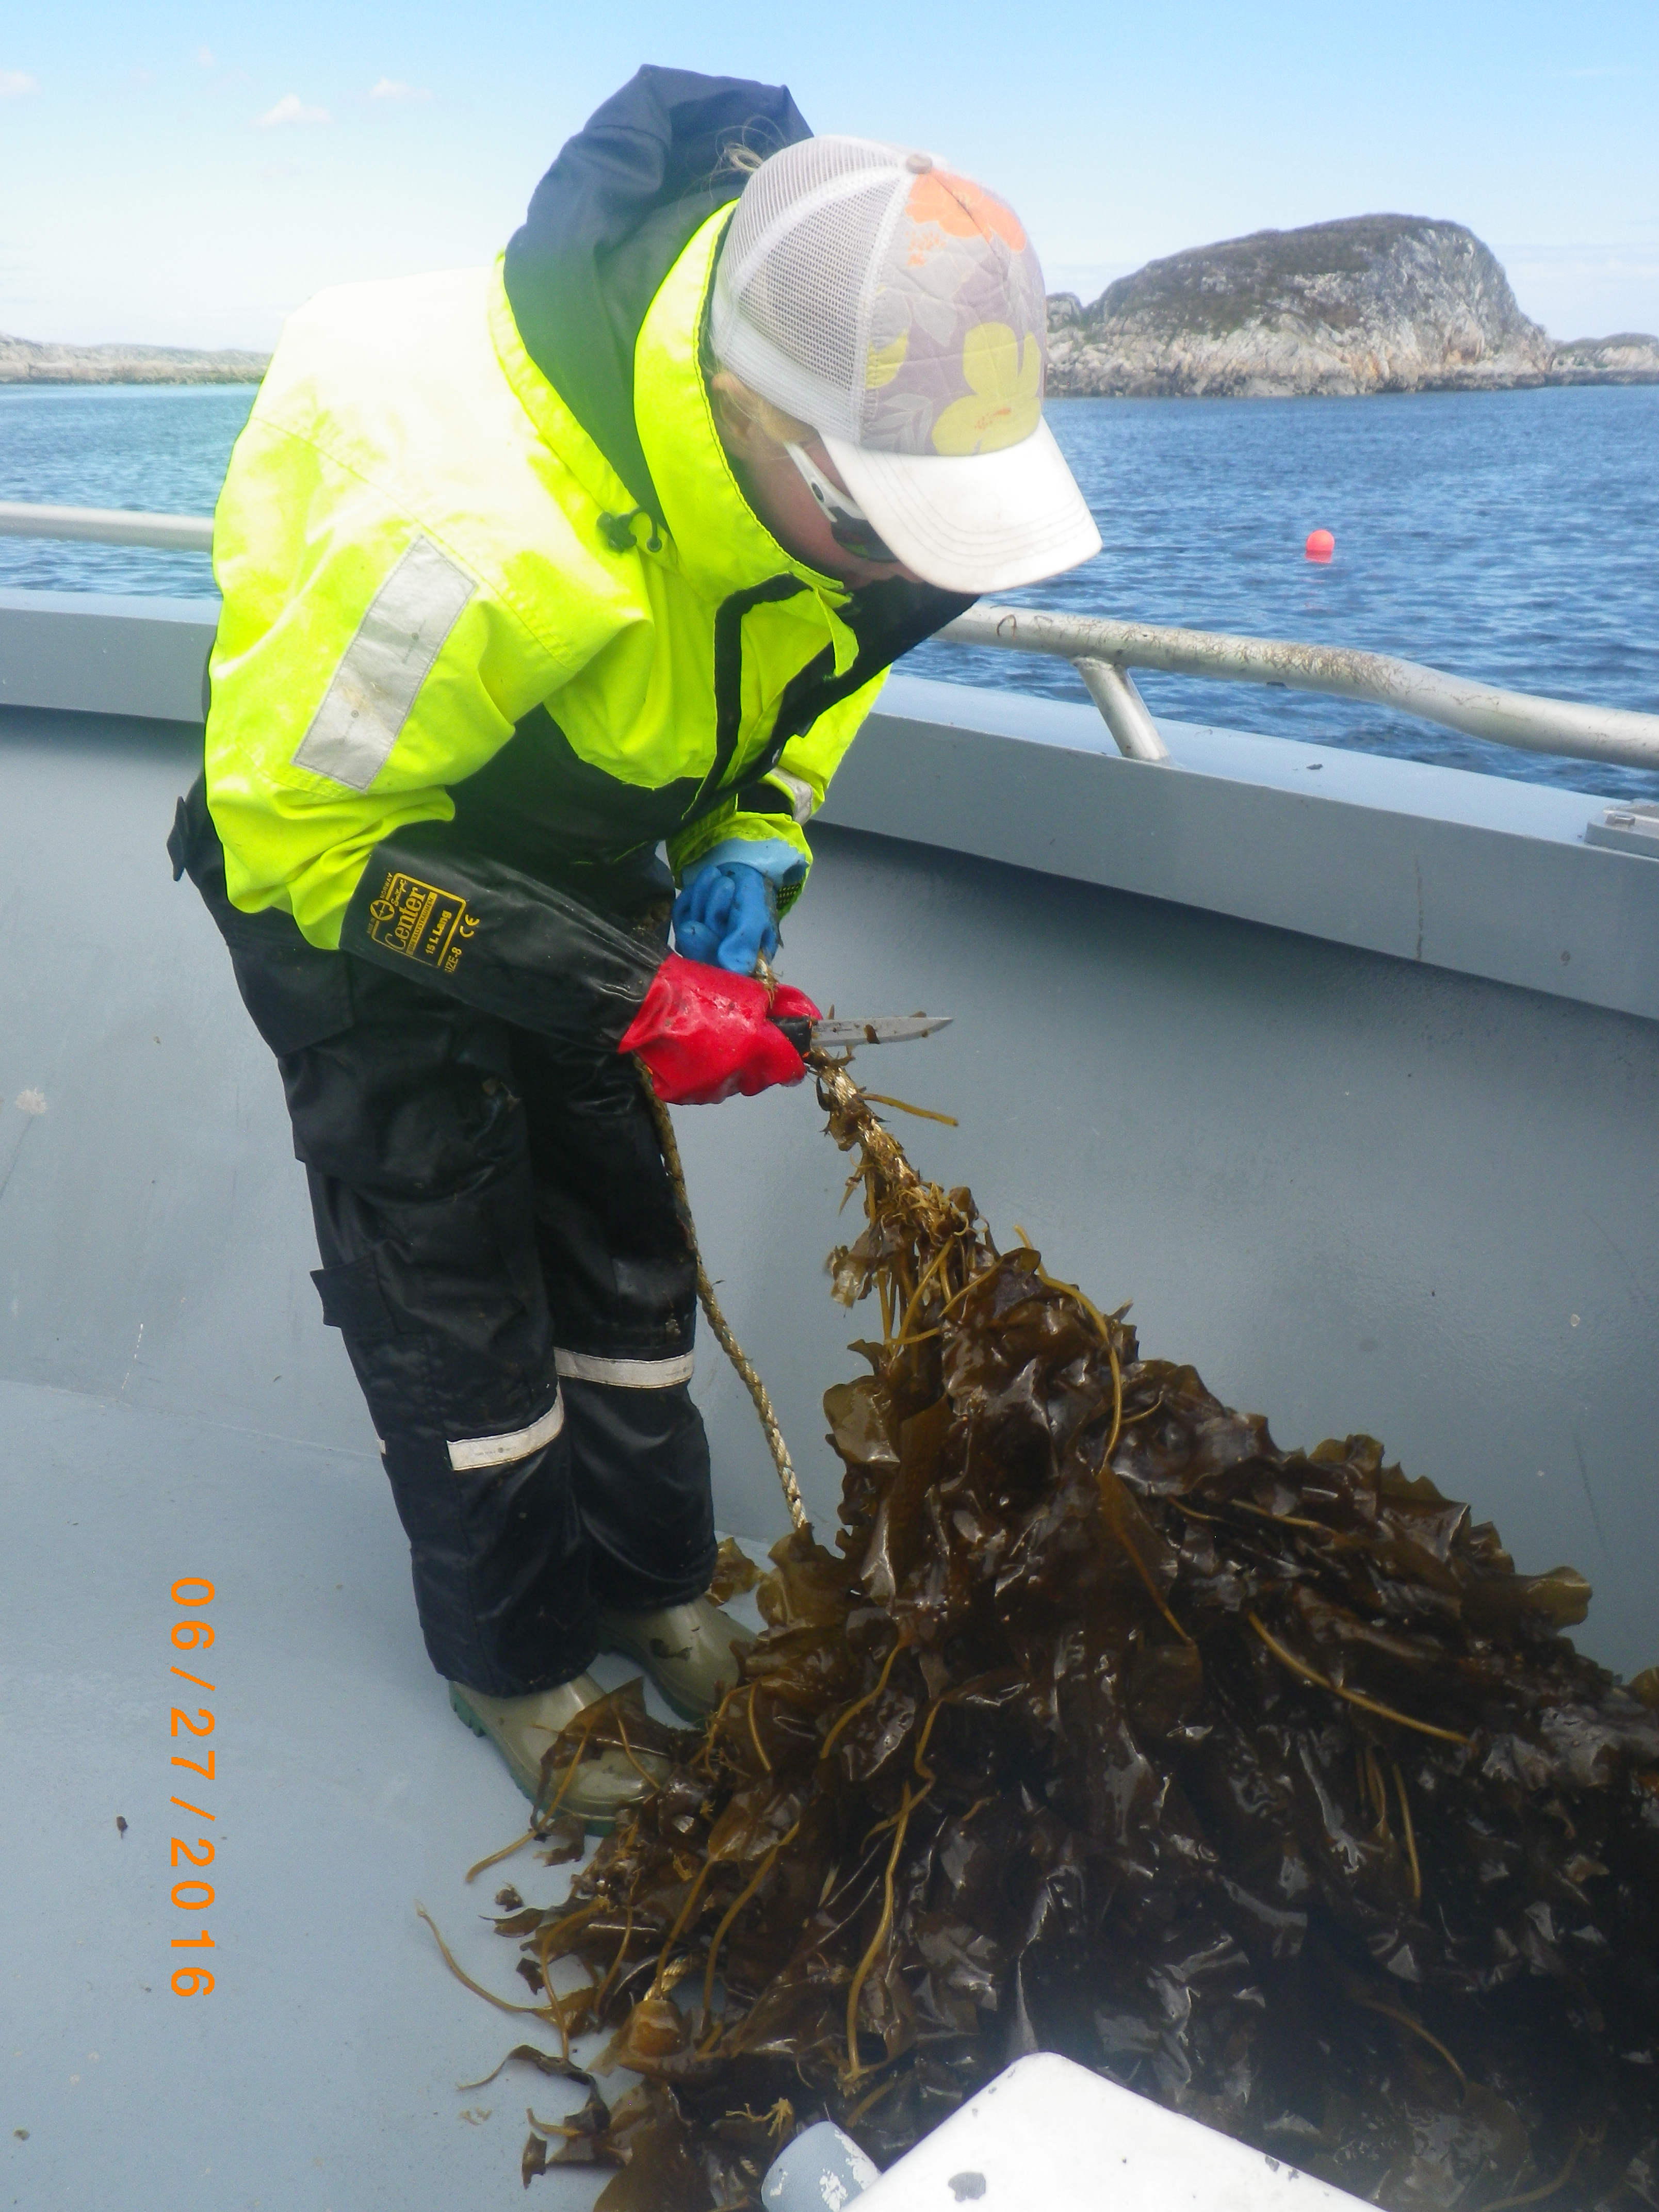
\includegraphics[width=0.5\textwidth]{kelp_photo/sonja}
  \caption{\textit{Saccharina latissima} being harvested}
  \label{fig:sonja}
\end{figure}

Large scale macroalgae cultivation has long existed in Eastern Asia due to the popularity of seaweed in Asian cuisine, and low labor costs that facilitate its manual seeding and harvest.
  More recently, less labor-intense and more industrialized kelp aquaculture has been developing in Scandinavia and in the Northeastern United States and Canada.
  For example, the MACROSEA project is a four year international research collaboration led by SINTEF, an independent research organization in Norway, and funded by the Research Council of Norway.
  The project's aim is to achieve ``successful and predictable production of high quality biomass thereby making significant steps towards industrial macroalgae cultivation in Norway''.
Figure \ref{fig:sonja} shows seaweed being harvested onboard a SINTEF research vessel.
The project includes both cultivators and scientists, working to develop a precise understanding of the full life cycle of kelp and its interaction with its environment.

A fundamental aspect of this endeavor is the development of mathematical models to describe the growth of kelp.
The development of mathematical models enables insight into a system which would be otherwise difficult or impossible to obtain.
For example, imagine that a company is interested in a new IMTA site, and is looking for a suitable location.
Running simulations to predict the potential productivity of each area would be of great assistance in choosing the best site.
Similarly, if a new cultivation technique is under consideration, simulation can estimate its viability without
having to deploy it on a large scale and risk failure or avoidable inefficiency.

Recently, a growth model \cite{broch_modelling_2012} for \textit{S. latissima} has been produced and integrated into the SINMOD \cite{wassmann_modelling_2006} hydrodynamic and ecosystem model of SINTEF.
This kelp model considers factors such as temperature, nutrient concentration, light availability, and water current.
The amount of light available is informed by spatially varying attenuation coefficients from SINMOD,
which considers optical properties of the water as well as concentrations of various organic and inorganic constituents.
However, it does not consider the effect of the kelp itself on the light field.
This is an important consideration, as high kelp densities should lead to low light levels which would inhibit further growth.
However, without accounting for self-shading, the kelp is not adequately penalized for growing too densely,
which is expected to cause overpredictions in the total biomass production.
The purpose of this thesis is to develop a first principles light model which adequately predicts the effects of self-shading on seaweed.


\section{Background on Kelp Models}

Mathematical modeling of macroalgae growth is not a new topic, although it is a reemerging one.
Several authors in the second half of the twentieth century were interested in describing the growth and composition of the macroalgae \textit{Macrocystis pyrifera}, commonly known as ``giant kelp,'' which grows prolifically off the coast of southern California.
The first such mathematical model was developed by W.J. North for the Kelp Habitat Improvement Project at the California Institute of Technology in 1968 using seven variables.
By 1974, Nick Anderson greatly expanded on North's work, and created the first comprehensive model of kelp growth which he programmed using FORTRAN \cite{anderson_mathematical_1974}.
In his model, he accounts for solar radiation intensity as a function of time of year and time of day, and refraction on the surface of the water.
He uses a simple model for shading, specifying a single parameter which determines the percentage of light that is allowed to pass through the kelp canopy floating on the surface of the water.
He also accounts for attenuation due to turbidity using Beer's Law.
Using this data on the availability of light, he calculates the photosynthesis rates and the growth experienced by the kelp.

Over a decade later in 1987, G.A.
Jackson expanded on Anderson's model for \textit{Macrocystis pyrifera} \cite{jackson_modelling_1987}, with an emphasis on including more environmental parameters and a more complete description of the growth and decay of the kelp.
The author takes into account respiration, frond decay, and sub-canopy light attenuation due to self-shading.
Light attenuation is represented with a simple exponential model, and self-shading appears as an added term in the decay coefficient.
The author does not consider radial or angular dependence on shading.
Jackson also expands Anderson's definition of canopy shading, treating the canopy not as a single layer, but as 0, 1, or 2 discrete layers, each composed of individual fronds.
While this is a significant improvement over Anderson's light model, it is still rather simplistic.

Both Anderson's and Jackson's model were carried out by numerically solving a system of differential equations over small time intervals.
In 1990, M.A. Burgman and V.A. Gerard developed a stochastic population model \cite{burgman_stage-structured_1990}.
This approach functions by dividing kelp plants into groups based on size and age and generating random numbers to determine how the population distribution over these groups changes over time based on measured rates of growth, death, decay, light availability, etc.
In the same year, Nyman et. al. \cite{nyman_macrocystis_1990} published a similar model alongside a Markov chain model, and compared the results with experimental data collected in New Zealand.

In 1996 and 1998 respectively, P. Duarte and J.G. Ferreira used the size-class approach to create a more general model of macroalgae growth, and Yoshimori et. al. created a differential equation model of \textit{Laminaria religiosa} with specific emphasis on temperature dependence of growth rate \cite{duarte_model_1997,yoshimori_mathematical_1998}.
These were some of the first models of kelp growth that did not specifically relate to \textit{Macrocystis pyrifera} (``giant kelp'').

The model developed by Broch et. al. at SINTEF \cite{broch_modelling_2012, broch_modelling_2013, handa_seasonal_2013} uses a super-individual approach, whereby a small number of individual kelp fronds are explicitly simulated at several discrete depth layers.
Each super-individual is assumed to represent a certain number of actual individuals in the population.
The number of individuals represented by each super-individual may change over the course of the simulation due to population loss.
The super-individual approach has the advantage of capturing some of the dynamics at the individual scale, while compromising full detail for the sake of reduced computational cost.

\section{Background on Radiative Transfer}
In terms of optical quantities, of primary interest is the radiance, which describes the rate of energy flow through each point in space in \textit{each} direction.
Irradiance, on the other hand, describes the total energy flow through a point in space over \textit{every} direction, and is calculated by integrating radiance over all angles.
Irradiance, in turn, determines the photosynthetic rate of the kelp, and therefore the total amount of biomass producible in a given area as well as the total nutrient remediation potential.
The equation governing the radiance throughout the system is known as the radiative transfer equation (RTE), which has been used extensively in stellar astrophysics \cite{chandrasekhar_radiative_1960,petkova_novel_2011}; its application to marine biology is fairly recent \cite{mobley_radiative_2001}.
In its full form, radiance is a function of 3 spatial dimensions, 2 angular dimensions, and frequency, making for a formidable problem.
In this work, frequency is ignored; only the total radiation in the photosynthetic spectrum, known as photosynthetically active radiation (PAR), is considered.
The RTE states that along a given path, radiance is decreased by absorption and scattering out of the path, while it is increased by emission and scattering into the path.
In the case of macroalgae cultivation, emission is negligible, owing only perhaps to some small luminescent phytoplankton or other anomaly, and can therefore be safely ignored.
However, the emission term will be retained in the calculations of this thesis, as it is mathematically useful to verify the correctness of the solution algorithm.

\section{Overview of Thesis}
The remainder of this document is organized as follows.
In Chapter \Rom{\ref{chap:kelp}}, a probabilistic model is developed to describe the spatial distribution of kelp by assuming simple distributions for the lengths and orientations of fronds.
Chapter \Rom{\ref{chap:light}} begins with a survey of fundamental radiometric quantities and optical properties of matter.
The spatial kelp distribution from Chapter \Rom{\ref{chap:kelp}} is used to determine optical properties of the combined water-kelp medium,
and the radiative transfer equation, an integro-partial differential equation which describes the the light field as a function of position and angle, is discussed.
An asymptotic expansion is explored for the case of low scattering, allowing for analytical, ordered approximations to the true light field.
In Chapter \Rom{\ref{chap:numerical}}, details are given for the numerical solution of the equations from Chapters \Rom{\ref{chap:kelp}} and \Rom{\ref{chap:light}}.
Both the full finite difference solution and the asymptotic approximation are thoroughly developed.

Chapter \Rom{\ref{chap:model_analysis}} is an in--depth discussion of sources of error in both solution procedures.
The concepts of verifying codes in general as well as specific calculations are discussed.
Exact discretization errors are calculated via the method of manufactured solutions in order to demonstrate
that the methods exhibit convergence properties which build confidence in their correctness.
A method for estimating errors for realistic cases is also developed.

Next, Chapter \Rom{\ref{chap:application}} surveys practical considerations to keep in mind when applying the algorithms in real situations.
Relevant model parameter values from the literature are collected, and estimates are given for those not readily available.
Following that is a set of guidelines for choosing which algorithm and which algorithm parameters to use based on the optical scenario to be simulated.
Advantages and disadvantages of both approaches are presented.
While the finite difference technique can be applied to any situation, it often requires prohibitively large CPU and memory resources, whereas the numerical asymptotic solution is generally faster and its memory footprint never exceeds the capacity of a standard laptop for reasonable grid sizes.
The Chapter concludes with a comparison to other two simpler light models, and specific qualitative differences are noted.
As expected, the presence of self-shading in this model results in the prediction of lower light levels regions of high kelp density.
However, the presence of scattering in the model increases light levels elsewhere, especially near the surface of the water.

Finally, Chapter \Rom{\ref{chap:conclusion}} concludes the thesis by briefly summarizing the model, discussing its achievements and limitations, and suggesting improvements and avenues for future work.
Several appendices follow with further details about the algorithm, as well as the full source code of the Fortran model developed.

\chapter{KELP MODEL}
\label{chap:kelp}

In order to properly model the spatial distribution of light around the kelp, it is first necessary to formulate a spatial description of the kelp.
Probability distributions are given for the size and orientation of the individual kelp fronds, which are inverted to determine the probability of a point in space being occupied by kelp.
Ultimately, the kelp density at any point in space is calculated, which informs the absorption coefficient of the effective kelp--water medium.


\section{Physical Setup}
The life of cultivated macroalgae generally begins in the laboratory, where microscopic kelp spores are inoculated onto a thread in a small laboratory pool.
This thread is wrapped around a larger rope as in Figure \ref{fig:rope_thread}, which is hung from buoys in the ocean.
The two primary configurations are vertical and horizontal or ``long'' lines.
In the case of vertical lines, the seaweed rope hangs straight down from a single buoy, and is either weighted or anchored.
In the case of long lines, the rope is strung from one buoy to another.
Long lines allow more light to reach the seaweed since it grows closer to the surface, but more vertical lines can be set up in a given area,
which may be advantageous for IMTA.

\begin{figure}[H]
  \centering
  \includegraphics[width=0.65\textwidth]{kelp_photo/rope_thread}
  \caption{\textit{Saccharina latissima} innoculated onto a thread wrapped around a rope on which it is to be grown.}
  \label{fig:rope_thread}
\end{figure}

We consider only the case of a rigid vertical rope which does not sway in the current.
The mature \textit{Saccharina latissima} plant consists of a single frond (leaf), a stipe (stem) and a holdfast (root structure).
For the sake of this model, only the kelp frond is considered, and its base is attached directly to the rope.
The ``gentle undulation approximation'' is employed, whereby it is assumed that fronds are on modeled as perfectly horizontal.
While at any given time they may point up or down due to water current and gravity, we consider the horizontal
state to be an average configuration.
This simplification allows for the three-dimensionally distributed population of kelp fronds
to be considered a collection of independent populations in two-dimensional depth layers.
A computer rendering of this scenario is shown in Figure \ref{fig:kelp_array}.

\begin{figure}[H]
	\centering
	\includegraphics[width=3.5in]{kelp_array}
	\captionof{figure}{Rendering of four nearby vertical kelp ropes as represented in the spatial distribution model. Note the kite--shaped fronds and horizontal orientation.}
  \label{fig:kelp_array}
\end{figure}

\section{Coordinate System}
Consider the rectangular domain
\begin{align*}
  \xmin &\leq x \leq \xmax, \\
  \ymin &\leq y \leq \ymax, \\
  \zmin &\leq z \leq \zmax.
\end{align*}
For all three dimensional analysis, we use the absolute coordinate system defined in Figure \ref{fig:3dcoords}.
In the following sections, it is necessary to convert between Cartesian and spherical coordinates, which we do using the relations
\begin{equation}
  \left\{
	\begin{split}
		x & = r\sin\phi\cos\theta, \\
		y & = r\sin\phi\sin\theta, \\
		z & = r\cos\phi. \\
	\end{split}
  \right.
	\label{eqn:coords}
\end{equation}
Therefore, for some function $f(x,y,z)$, we can write its derivative along a path in spherical coordinates in terms of Cartesian coordinates using the chain rule,
\begin{equation*}
	\frac{\partial f}{\partial r}
	=\frac{\partial f}{\partial x}\frac{\partial x}{\partial r}
	+ \frac{\partial f}{\partial y}\frac{\partial y}{\partial r}
	+ \frac{\partial f}{\partial z}\frac{\partial z}{\partial r}.
\end{equation*}
Then, calculating derivatives from \eqref{eqn:coords} yields
\begin{equation}
	\frac{\partial f}{\partial r}
	=\frac{\partial f}{\partial x}\sin\phi\cos\theta
	+ \frac{\partial f}{\partial y}\sin\phi\sin\theta
	+ \frac{\partial f}{\partial z}\cos\phi.
	\label{eqn:partials}
\end{equation}
\begin{figure}[H]
	\centering
	\includegraphics[width=3in]{3d_coords}
	\caption{Downward-facing right-handed coordinate system with radial distance $r$ from the origin, distance $s$ from the $z$ axis, zenith angle $\phi$ and azimuthal angle $\theta$.}
	\label{fig:3dcoords}
\end{figure}

\section{Population Distributions}
In order to construct a spatial distribution of kelp fronds, a simple kite-shaped geometry is introduced,
and frond lengths and azimuthal orientations are assumed to be distributed predictably.
Since it is assumed that fronds extend perfectly horizontally, no angular elevation distribution is required.

\subsection{Frond Shape}
\label{sec:shape}

\begin{figure}[h]
	\centering
  \includegraphics[width=1.2in]{kelp_photo/kite}
  %TODO: Cite this?
  \qquad
	\includegraphics[width=2in]{frond}
	\captionof{figure}{Simplified kite-shaped frond.}
	\label{fig:frond}
\end{figure}

The frond is assumed to be kite-shaped with length $l$ from base to tip, and width $w$ from left to right.
In Figure \ref{fig:frond}, the base is shown at the bottom and the tip is shown at the top.
The proximal length is the shortest distance from the base to the diagonal connecting the left and right corners, and is notated as $f_a$.
Likewise, the distal length, notated $f_b$, is the shortest distance from that diagonal to the tip.
It is therefore clear that
 \begin{equation*}
	 f_a + f_b = l.
 \end{equation*}
When considering a whole population with varying sizes, it is more convenient to specify ratios than absolute lengths.
Define the ratios
\begin{align*}
	f_r &= \frac{l}{w}, \\
	f_s &= \frac{f_a}{f_b}.
\end{align*}
These ratios are assumed to be constant among the entire population, so that all fronds are geometrically similar.
Thus, the shape of the frond can be fully specified by $l$, $f_r$, and $f_s$;
it is possible to redefine $w$, $f_a$ and $f_b$ from the preceding formulas as
\begin{align*}
	w &= \frac{l}{f_r}, \\
	f_a &= \frac{lf_s}{1+f_s}, \\
	f_b &= \frac{l}{1+f_s}.
\end{align*}
The angle $\alpha$, half of the angle at the base corner, is also noteworthy.
From the above equations, it follows that
\begin{equation*}
	\alpha = \tan^{-1}\left(\frac{2f_rf_s}{1+f_s}\right).
\end{equation*}

It is useful to convert between frond length and surface area, which can be done via the relations
\begin{align}
  A &= \frac{lw}{2} = \frac{l^2}{2f_r}, \\
  l &= \sqrt{2Af_r}.
  \label{eqn:length-from-area}
\end{align}

\subsection{Length and Angle Distributions}
\label{sec:dist}
In any given depth layer, the distribution of frond lengths is assumed to be normal, with mean $\mu_l$ and standard deviation $\sigma_l$.
That is, it has the probability density function (PDF)
\begin{equation*}
  P_l(l) = \frac{1}{\sqrt{2\pi\sigma_l^2}}\exp\left(\frac{(l-\mu_l)^2}{2\sigma_l^2}\right).
\end{equation*}

It is further assumed that frond orientation angle varies according to the von Mises distribution, which is the periodic analogue of the normal distribution, defined on $[-\pi,\pi]$ rather than $(-\infty,\infty)$.
The von Mises distribution has two parameters, $\mu$ and $\kappa$, which shift and sharpen its peak respectively, as shown in Figure \ref{fig:vonmises}.
$\kappa$ is analogous to $1/\sigma$ in the normal distribution.
In the absence of current, the frond angles are distributed uniformly, while as current velocity increases, they become increasingly likely to align parallel to the current, depending on the stiffness of the frond and stipe.
Assuming a linear relationship between the current velocity and the steepness of the angular distribution, define the \textit{frond alignment coefficient} $\eta$, with units of inverse velocity(\SI{}{\s\per\m}).
Then, use $\mu = \theta_w$ and $\kappa = \eta v_w$ as the von Mises distribution parameters.
Note that $\theta_w$ and $v_w$ vary over depth, while $\eta$ is assumed constant for the population.
Then, the PDF for the von Mises frond angle distribution is
\begin{equation*}
	P_{\theta_f}(\theta_f) = \frac{\exp\left(\eta v_w\cos(\theta_f-\theta_w)\right)}{2\pi I_0(\eta v_w)},
\end{equation*}
where $I_0(x)$ is the modified Bessel function of the first kind of order 0.
Notice that unlike the normal distribution, the von Mises distribution approaches a \textit{non-zero} uniform distribution as $\kappa$ approaches 0, so
\begin{equation*}
	\displaystyle \lim_{v_w \to 0}P_{\theta_f}(\theta_f) = \frac{1}{2\pi} \;\forall\, \theta_f \in [-\pi,\pi].
\end{equation*}

\begin{figure}[h]
	\centering
	\includegraphics[width=6in]{vonmises}
	\captionof{figure}{von Mises distribution for a variety of parameters.}
	\label{fig:vonmises}
\end{figure}

\subsection{Joint Length-Orientation Distribution}
\label{sec:dist_2d}
The previous two distributions can reasonably be assumed to be independent of one another. That is, the angle of the frond does not depend on the length, or vice versa.
Therefore, the probability of a frond simultaneously having a given frond length and angle is the product of their individual probabilities.
Given independent events $A$ and $B$, the probability of their intersection is the product of their individual probabilities.
That is,
\begin{equation*}
	\label{eq:ind_prob}
	P(A \cap B) = P(A)P(B).
\end{equation*}
Then the probability of frond length $l$ and frond angle $\theta_f$ coinciding is
\begin{equation}
  \label{eq:p2d}
	P_{2D}(\theta_f,l) = P_{\theta_f}(\theta_f) \cdot P_l(l).
\end{equation}
A contour plot of this 2D distribution for a specific set of parameters is shown in Figure \ref{fig:dist_2d}, where probability is represented by color in the 2D plane.
Darker green represents higher probability, while lighter beige represents lower probability.
In Figure \ref{fig:kelp_sample}, 50 samples are drawn from this distribution and plotted.

It is important to note that if $P_{\theta_f}$ were dependent on $l$, the above definition of $P_{2D}$ would no longer be valid.
For example, it might be more realistic to say that larger fronds are less likely to bend towards the direction of the current.
In this case, \eqref{eq:ind_prob} would no longer hold, and it would be necessary to use the more general Bayes' Theorem
\begin{equation*}
	P(A \cap B) = P(A)P(B|A) = P(B)P(B|A),
\end{equation*}
which is currently not taken into consideration in this model.

\begin{figure}[h]
	\centering
	\includegraphics[width=4.5in]{prob_2d}
	\captionof{figure}{2D length-angle probability distribution with $\theta_w=7\pi/4$, $v_w=1$, $\mu_l=3$, $\sigma_l=1$.}
	\label{fig:dist_2d}
\end{figure}

\begin{figure}[h]
	\centering
	\includegraphics[width=4.5in]{kelp_sample}
	\captionof{figure}{A sample of 50 kelp fronds with shape parameters $f_s=0.5$ and $f_r=2$ whose lengths are picked from a normal distribution and whose angles are picked from a von Mises distribution.}
	\label{fig:kelp_sample}
\end{figure}

\section{Spatial Distribution}
In this section, the population length and angle distributions from the previous section are used to construct a spatial distribution of kelp.
This is made possible by the simple kite-shape fronds, and would be considerably more difficult with more general frond shapes.
\subsection{Rotated Coordinate System}
\label{sec:rot_coords}
To determine under what conditions a frond will occupy a given point, we begin by
describing the shape of the frond in Cartesian coordinates and then convert to polar coordinates.
Of primary interest are the edges connected to the frond tip.
For convenience, we will use a rotated polar coordinate system $(\theta',s)$ such that the line connecting the base to the tip points in the $+y$ direction ($\theta=\pi/2$), with the base at $(0,0)$.
Denote the Cartesian analogue of this coordinate system as $(x',y')$ which is related to $(\theta',s)$ by
\begin{align*}
	x' &= s\cos\theta' \\
	y' &= s\sin\theta' \\
	s &= \sqrt{x'^2+y'^2}, \\
	\theta' &= \atantwo(y, x).
\end{align*}

\subsection{Functional Description of Frond Edge}
With this coordinate system established, the outer two edges of the frond can be described in Cartesian coordinates as a piecewise linear function connecting the left corner: $(-w/2,f_a)$, the tip: $(0,l)$, and the right corner: $(w/2,f_a)$.
This function has the form
\begin{equation*}
	y'_f(x') = l-\sign(x')\frac{f_b}{w/2}x'.
\end{equation*}
Using the equations in Section \ref{sec:rot_coords}, this can be written in polar coordinates after some rearrangement as
\begin{equation*}
	s_f'(\theta';l) = \frac{l}{\sin\theta' + S(\theta')\frac{2f_b}{w}\cos\theta'},
\end{equation*}
where
\begin{equation*}
	S(\theta') = \sign(\cos\theta').
\end{equation*}
Then, using the relationships in Section \ref{sec:shape}, the above equation can be rewritten in terms of the frond ratios $f_s$ and $f_r$ as
\begin{equation}
	\label{eq:rf_rel}
	s_f'(\theta';l) = \frac{l}{\sin\theta' + S(\theta')\frac{2f_r}{1+f_s}\cos\theta'}.
\end{equation}
For convenience, denote the denominator of \eqref{eq:rf_rel} as $d_f'(\theta')$.
To generalize to a frond pointed at an angle $\theta_f$, we introduce the coordinate system $(\theta,s)$ such that
\begin{equation*}
	\theta = \theta' + \theta_f - \frac{\pi}{2}.
\end{equation*}
Then, for a frond pointed at the arbitrary angle $\theta_f$, the function for the outer edges can be written as
\begin{equation}
	\label{eq:rf_abs}
	s_f(\theta;l) = s_f'\left(\theta - \theta_f + \frac{\pi}{2} \right).
\end{equation}
Similarly, define
\begin{equation}
	d_f(\theta) = d_f'\left(\theta - \theta_f + \frac{\pi}{2} \right).
\end{equation}

\subsection{Conditions for Occupancy}
We now formulate the conditions under which a kite shape frond occupies a point
in the sense that the point lies within its interior.
Combining these conditions with the size and orientation distributions from \ref{sec:dist}
allows a spatial distribution of the kelp fronds to be calculated.

Consider a fixed frond of length $l$ at an angle $\theta_f$. The point
$(\theta,s)$ is occupied by the frond if
\begin{align*}
	\left|\theta_f - \theta \right| < \alpha
  \mbox{ and }
	s < s_f(\theta).
\end{align*}
Equivalently, the opposite perspective can be taken.
Letting the point $(\theta,s)$ be fixed, a frond occupies the point if
\begin{align}
	\theta - \alpha < \theta_f < \theta + \alpha,
	\label{eqn:rs_th} \\
	l > l_{\min}(\theta,s),
	\label{eqn:rs_l}
\end{align}
where
\begin{equation*}
	l_{\min}(\theta,s) = s \cdot \frac{l}{s_f(\theta;l)} = s \cdot d_f(\theta).
\end{equation*}
Then, considering the point to be fixed, \eqref{eqn:rs_th} and \eqref{eqn:rs_l} define the spacial region $R_s(\theta,s)$ called the ``occupancy region for $(\theta,s)$'' with the property that if the tip of a frond lies within this region (i.e., $(\theta_f,l) \in R_s(\theta,s)$), then it occupies the point.
$R_s(3\pi/4,1.5)$ is shown in blue in Figure \ref{fig:shade_area} and the smallest possible occupying fronds for several values of $\theta_f$ are shown in various colors.
Any frond longer than these at the same angle will also occupy the point.

\begin{figure}[h]
	\centering
	\includegraphics[width=4.5in]{shade_area}
	\captionof{figure}{Outlines of minimum-length fronds for a variety of angles to occupy the point $(\theta,s)=(3\pi/4,3/2)$.}
	\label{fig:shade_area}
\end{figure}

\subsection{Probability of Occupancy}
We are interested in the probability that, given a fixed point $(\theta,s)$, values of $l$ and $\theta_f$ chosen from the distributions described in Section \ref{sec:dist} will fall in the occupancy region.
This is found by integrating $P_{2D}(\theta_f, l)$ from \eqref{eq:p2d} over $R_s(\theta,s)$, the occupancy region for the point of interest.

\begin{figure}[h]
	\centering
	\includegraphics[width=4.5in]{cart_shade}
	\captionof{figure}{Contour plot of $P_{2D}(\theta_f,l)$ overlayed with the
    region in the $\theta_f$\nobreak--\nobreak$l$ plane which results in a frond occupying the point $(\theta,s)=(3\pi/4,3/2)$.}
	\label{fig:cart_shade}
\end{figure}

Integrating $P_{2D}(\theta_f,l)$ over $R_s(\theta,s)$ as depicted in Figure \ref{fig:cart_shade} yields the proportion of the population in the depth layer occupying the point $(\theta,s)$,
\begin{align*}
		\tilde{P}_k(\theta,s,z)	&= \iint_{R_s(\theta,s)}
								P_{2D}(\theta_f,l)
								\,dl\,d\theta_f \nonumber \\
							&= \int_{\theta-\alpha}^{\theta+\alpha}
								\int_{l_{\min}(\theta_f)}^\infty
								P_{2D}(\theta_f,l)
								\,dl\,d\theta_f.
\end{align*}

Assuming that the depth layer has thickness $dz$ and contains $n$ fronds of thickness $t$,
the proportion of the vertical length of the discrete depth layer occupied by kelp at any position $(x,y,z)$ is given by
\begin{equation*}
  P_k(x, y) = \frac{nt}{dz}\tilde{P}_k(x, y).
\end{equation*}
In the continuum limit as the number of discrete depth depth layers approaches infinity, $P_k(x,y,z)$ can be interpreted as the probability of the point $(x,y,z)$ being occupied by kelp.
In a three dimensional context, the number of fronds is more likely to be specified by a number density $\rho_n=n/dz$ over the vertical length of the rope with units \SI{}{\per\m}, in which case
\begin{equation*}
  P_k(x, y, z) = t \rho_n(z) \tilde{P}_k(x, y, z).
\end{equation*}
Then, since the point $\vec{x}$ has a probability $P_k(\vec{x})$ of being occupied by kelp and a probability $(1-P_k(\vec{x}))$ of being occupied by the surrounding aquatic medium,
the effective absorption coefficient can be calculated as
\begin{equation*}
  a(\vec{x}) = P_k(\vec{x})a_k + (1-P_k(\vec{x}))a_w,
\end{equation*},
where $a_k$ is the absorption coefficient of the kelp alone, and $a_w$ is the absorption coefficient of the water and its dissolved and suspended contents.

\begin{figure}[h]
	\centering
	\includegraphics[width=4.5in]{prob_shade}
	\captionof{figure}{Contour plot of the probability of frond occupation sampled at 121 points using $\theta_f=2\pi/3,\eta v_w=1$.}
	\label{fig:prob_shade}
\end{figure}

\section{Discontinuity at the rope}
While the above model of the kelp distribution is straightforward to evaluate, it does have a significant numerical difficulty in its application.
Since the length and orientations are both continuous in the polar coordinates $s>0$ and $\theta$, the resulting kelp density and effective absorption coefficient are as well.
However, they are not necessarily continuous in Cartesian coordinates.
In the case of no water current, $v_w=0$, the flat von Mises distribution produces a continuous solution at the origin.
In the more general case, though, there is a high kelp density on one side of the origin in the direction of the current, and a low kelp density immediately on the other side.
Since rope is assumed to be infinitely thin and have a fixed position, the sharp corners of the kelp fronds eminate from exactly the same point.
Hence, there is in general a discontinuity in the kelp distribution at the origin, and therefore its derivatives are unbounded on the domain.

This is not appealing numerically since the algorithms used in this thesis to solve the differential equation describing the light field, are based on interpolation on a discrete Cartesian grid.
According to Taylor's theorem, the error incurred by performing such interpolation is bounded by a constant multiple of the appropriate maximum derivative of the interpolated function over the domain.
If the derivatives of the absorption coefficient are unbounded, then so too is the discretization error in the final solution.
That is, the solution is not guaranteed to converge.

Luckily, there is a straightforward solution, which is to post-process the spatial kelp distribution with a Gaussian blur in the $x$ and $y$ dimensions.
This is achieved via convolution of the solution with a 2D Gaussian kernel centered at the origin.
Any blur whatsoever is sufficient to bound the derivatives, and the larger the blur radius, the smaller they become.
Obviously, as the blur radius is increased, the kelp distribution tends toward a constant and no longer captures any information about the $xy$ distribution of the kelp.
Therefore, a small blur radius should be used.

\subsection{One dimensional Gaussian blur}
As a one dimensional analogy, consider the Heaviside step function,
\begin{equation*}
  H(x) = \begin{cases}
    0, & x < 0, \\
    1, & x > 0.
  \end{cases}
\end{equation*}
Clearly, the function is infinitely steep at the origin.
Consider the normalized Gaussian kernel centered at the origin with radius $\sigma_b$, given by
\begin{equation}
  k(x;\sigma_b) = \frac{1}{\sqrt{2\pi\sigma_b}^2} \exp\left({-\frac{x^2}{2\sigma_b^2}}\right).
\end{equation}
A blur is applied by convolving the function with the kernel according to the formula
\begin{align*}
  \tilde{H}(x) &= (k*H)(x) = \int_{-\infty}^{\infty}H(\tau)k(x-\tau;\sigma_b)\, d\tau \\
  &= \int_{0}^{\infty}k(x-\tau;\sigma_b)\, d\tau.
\end{align*}
The substitution $u=\tau=x,\, du=d\tau$ yields
\begin{equation*}
  \tilde{H}(x) = \int_{-x}^\infty k(u;\sigma_b)\, du.
\end{equation*}
Note that since the kernel is normalized, the integral from 0 to infinity is $1/2$.
Further, since the kernel is even, the integral over $[-x, 0]$ is equal to the integral over $[0, x]$.
Hence,
\begin{equation*}
  \tilde{H}(x) = \frac{1}{2} + \int_{0}^x k(u;\sigma_b)\, du.
\end{equation*}
Then, by the fundamental theorem of calculus, the derivative of the convolved function is simply $k(x;\sigma_b)$, whose maximum value is $k(0;\sigma_b) = 1/\sqrt{2\pi\sigma_b^2}$.
Then, since the derivative is a linear operator, this result can be generalized to the following statement:
Applying a Gaussian blur of radius $\sigma_b$ to a function with a maximum discontinuity of size $J$ produces a function whose first derivative is bounded by
\begin{equation*}
  \frac{1}{\sqrt{2\pi}}\frac{J}{\sigma_b}.
\end{equation*}
The same logic applies to directional derivatives of multidimensional scalar functions.

\subsection{Multidimensional Gaussian blur}
In light of the above arguments, the derivatives of the absorption coefficient are bounded by applying a two--dimensional Gaussian blur in $xy$--plane to $\tilde{P}_k$ using the kernel
\begin{equation}
  k(x, y; \sigma_b) = \frac{1}{\sqrt{2\pi\sigma_b^2}} \exp\left(\frac{x^2 + y^2}{2\sigma_b^2}\right).
\end{equation}
Hence, the blurred solution is
\begin{equation}
  \tilde{P}_k^b(x, y, z) = \int_{-\infty}^\infty \int_{-\infty}^\infty k(x-x', y-y', z; \sigma_b) \tilde{P}_k(x', y', z)\, dx'\, dy'.
\end{equation}

A physical interpretation of this Gaussian blurring is that $\tilde{P}_k^b$ is the time--averaged kelp distribution, assuming that the rope is allowed to move horizontally, and $k(x, y; \sigma)$ is the PDF of the rope's location distribution.
This interpretation is a bit incongruous with the rest of the model since there is no other explicit mention of time--averaging; while the frond length and position distributions can be thought of as continuous approximations to the population distribution at a single point in time, this idea does not apply to the rope's position, since there is only one.

\subsection{Absorption coefficient plots}
\begin{figure}[H]
  \centering
  \includegraphics[width=5in]{kelp_dist_sharp}
  \caption{Absorption coefficient profile in the limiting case of $v_w>>1$, $\sigma_l=0$ and $\sigma_b=0$ demonstrates the kite--shaped fronds. Note the high gradient near the inner edge of the frond.}
  \label{fig:kelp_dist_sharp}
\end{figure}
\begin{figure}[H]
  \centering
  \vspace{-3em}
  \includegraphics[width=5in]{kelp_dist_smooth}
  \caption{Absorption coefficient profile for realistic values of $v_w$ and $\sigma_l$, but with $\sigma_b=0$. Note the large gradient at the origin. By continuing to increase the plotting resolution, the gradient would be found to be unbounded.}
  \label{fig:kelp_dist_smooth}
\end{figure}
\begin{figure}[H]
  \centering
  \vspace{-3em}
  \includegraphics[width=5in]{kelp_dist_smooth_smallblur}
  \caption{A small blur radius of $\sigma_b=\SI{0.1}{\m}$ eliminates the derivative singularity at the origin.}
  \label{fig:kelp_dist_smooth_smallblur}
\end{figure}
\begin{figure}[H]
  \centering
  \vspace{-3em}
  \includegraphics[width=5in]{kelp_dist_smooth_blur}
  \caption{Over-blurring kelp distribution with $\sigma_b=\SI{10}{\m}$ causes it to lose a great deal of spatial resolution. This should be avoided.}
  \label{fig:kelp_dist_smooth_blur}
\end{figure}

\chapter{LIGHT MODEL}
\label{chap:light}

Now that we have formulated the distribution of kelp throughout the medium, we introduce the Radiative Transfer Equation, which is used to calculate the light field.

\section{Optical Definitions}
Before introducing the radiative transfer equation, it is necessary to discuss some basic radiometric quantities of interest which characterize the light field, as well as inherent optical properties which describe the medium of propagation.

\subsection{Radiometric Quantities}

One of the most fundamental quantities in optics is radiant flux $\Phi$, which is the has units of energy per time.
The quantity of primary interest in modeling the light field is radiance $L$, which is defined as the radiant flux per steradian per projected surface area perpendicular to the direction of propagation of the beam.
That is,
\begin{equation*}
	L = \frac{d^2\Phi}{dA d\vec{\omega}},
\end{equation*}
where $\vec{\omega}$ is an element of solid angle, and $A$ is an element of projected surface area.
Once the radiance $L$ is calculated everywhere, the irradiance is
\begin{equation*}
  I(\vec{x}) = \int_{4\pi}L(\vec{x},\vec{\omega})\, d\vec{\omega}.
\end{equation*}
Irradiance is sometimes given in units of moles of photons (a mole of photons is also called an Einstein) per second, with the conversion \cite{mobley_light_1994} given by
\begin{equation}
  \SI{1}{\W\per\m^2} = \SI{4.2}{\micro\mole \,photons\per\second}.
  \label{eqn:watts_photons}
\end{equation}

\subsection{Perceived Irradiance}
\label{sec:perceived_irrad}

The average irradiance experienced by a kelp frond in depth layer $k$ is
\newcommand{\Iperk}{\tilde{I}_k}
\begin{equation*}
   \Iperk = \frac{\sum_{ij}P_{ijk}I_{ijk}}{\sum_{ij}P_{ijk}}.
\end{equation*}
The irradiance perceived by the kelp is expected to be slightly lower than the average irradiance,
\begin{equation*}
  \bar{I}_k = \frac{\sum_{ij}I_{ijk}}{n_x n_y},
\end{equation*}
since the kelp is more densely located at the center of the domain where the light field is reduced,
whereas the simple average is influenced by regions of higher irradiance at the edges of the domain where kelp is not present.

\subsection{Inherent Optical Properties}
% TODO: Edit
We now define a few inherent optical properties (IOPs) which depend only on the medium of propagation.
These phenomena are governed by three inherent optical properties (IOPs) of the
medium.
The absorption coefficient $a(\vec{x})$ (units m$^{-1}$) defines the
proportional loss of radiance per unit length.
The scattering coefficient $b$ (units m$^{-1}$), defines the proportional loss
of radiance per unit length, and is assumed to be constant over space.

The volume scattering function (VSF) $\beta(\Delta): [-1, 1] \to \RR^+$ (units sr$^{-1}$) defines the probability of light scattering at any given angle from its source.
Formally, given two directions $\vec{\omega}$ and $\vec{\omega}'$, $\beta(\vec{\omega} \cdot \vec{\omega}')$ is the probability density of light scattering from $\vec{\omega}$ into $\vec{\omega}'$ (or vice-versa).
Of course, since a single direction subtends no solid angle, the probability of scattering occurring exactly from $\vec{\omega}$ to $\vec{\omega}'$ is 0.
Rather, we say that the probability of radiance being scattered from a direction $\omega$ into an element of solid angle $\Omega$ is $\int_\Omega \beta(\vec{\omega} \cdot \vec{\omega}')\, d\vec{\omega}'$.

The VSF is normalized such that
\begin{equation*}
  \int_{-1}^1\beta(\Delta)\, d\Delta=\frac{1}{2\pi},
\end{equation*}
so that for any $\omega$,
\begin{equation*}
  \int_{4\pi}\beta(\vec{\omega}\cdot\vec{\omega}')\, d\vec{\omega}' = 1.
\end{equation*}
i.e., the probability of light being scattered to some direction on the unit sphere is 1.


\section{The Radiative Transfer Equation}
% TODO: Blurb
We now present the Radiative Transfer Equation, whose solution is the radiance in the medium as a function of position and angle.

\subsection{Ray Notation}
Consider a fixed position $\vec{x}$ and direction $\vec{\omega}$ such that
$\vec{\omega} \cdot \hat{z} \neq 0$.
% TODO: Just call $\vec{x_0}$ a point, not a function. Call it the projection to the surface.
Let $\vec{l}(\vec{x}, \vec{\omega}, s)$ denote the linear path containing $\vec{x}$ in the direction $\vec{\omega}$.
Assume that the ray is not horizontal.
Then, it originates either at the surface or bottom of the domain, with initial z coordinate given by
\begin{equation*}
  z_0 =
   \begin{cases}
    0, & \vec{\omega} \cdot \hat{z} < 0 \\
    \zmax, & \vec{\omega} \cdot \hat{z} > 0.
  \end{cases}
\end{equation*}
Hence, the ray path is parameterized as
\begin{equation}
  \vec{l}(\vec{x}, \vec{\omega}, s) = \frac{1}{\tilde{s}} (s\vec{x} + (\tilde{s} - s)\vec{x_0}(\vec{x}, \vec{\omega})),
  \label{eqn:ray_path}
\end{equation}
where
\begin{equation*}
  \vec{x_0}(\vec{x}, \vec{\omega}) = \vec{x} - \tilde{s} \vec{\omega}
\end{equation*}
is the origin of the ray, and 
\begin{equation*}
  \tilde{s} = \frac{\vec{x} \cdot \hat{z} - z_0}{\vec{\omega} \cdot \hat{z}}
\end{equation*}
is the path length from $\vec{x_0}(\vec{x}, \vec{\omega})$ to $\vec{x}$.

\subsection{Colloquial Description}
Denote the radiance at $\vec{x}$ in the direction $\vec{\omega}$ by $L(\vec{x}, \vec{\omega})$.
As light travels along $\vec{l}(\vec{x}, \vec{\omega}, s)$, interaction with the
medium produces three phenomena of interest:
\begin{enumerate}
  \item Radiance is decreased due to absorption.
  \item Radiance is decreased due to scattering out of the path to other
    directions.
  \item Radiance is increased due to scattering into the path from other
      directions.
\end{enumerate}

\subsection{Equation of Transfer}
Combining these phenomena yields the Radiative Transfer Equation along
$\vec{l}(\vec{x}, \vec{\omega})$,
\begin{equation}
  \label{eqn:rte1d}
  \frac{dL}{ds}(\vec{l}(\vec{x}, \vec{\omega}, s), \vec{\omega})
  = -(a(\vec{x}) + b)L(\vec{x}, \vec{\omega})
  + b \int_{4\pi} \beta(\vec{\omega}\cdot\vec{\omega}') L(\vec{x})\, d\vec{\omega}',
\end{equation}
where $\int_{4\pi}$ denotes integration over the unit sphere.
The derivative of $L$ over the path can be rewritten as
\begin{align*}
  \frac{dL}{ds}(\vec{l}(\vec{x}, \vec{\omega}, s), \vec{\omega})
    &= \frac{d\vec{l}}{ds}(\vec{x}, \vec{\omega}, s) \cdot \nabla L(\vec{x}, \vec{\omega}', \vec{\omega}) \\
    &= \vec{\omega} \cdot \nabla L(\vec{x}, \vec{\omega}),
\end{align*}
which unveils the general form of the Radiative Transfer Equation,
\begin{equation*}
  \vec{\omega} \cdot \nabla L(\vec{x}, \vec{\omega})
  = -(a(\vec{x}) + b)L(\vec{x}, \vec{\omega})
  + b \int_{4\pi} \beta(\vec{\omega}\cdot\vec{\omega}') L(\vec{x}, \vec{\omega}')\, d\vec{\omega}'
\end{equation*}

or, equivalently,
\begin{equation}
  \vec{\omega} \cdot \nabla L(\vec{x}, \vec{\omega})
  + a(\vec{x})L(\vec{x}, \vec{\omega})
  = b \left(
    \int_{4\pi} \beta(\vec{\omega}\cdot\vec{\omega}') L(\vec{x}, \vec{\omega}')\, d\vec{\omega}'
    - L(\vec{x}, \vec{\omega})
  \right).
  \label{eqn:rte}
\end{equation}

\subsection{Boundary Conditions}

We use periodic boundary conditions in the $x$ and $y$ directions,
\begin{align*}
  L\left((\xmin, y, z), \vec{\omega}\right) &= L\left((\xmax, y, z), \vec{\omega}\right), \\
  L\left((x, \ymin, z), \vec{\omega}\right) &= L\left((x, \ymax, z), \vec{\omega}\right).
\end{align*}
In the $z$ direction, we specify a spatially uniform downwelling light just
under the surface of the water by a function $f(\vec{\omega})$.
Or if $\zmin>0$, then the radiance at $z=\zmin$ should be specified instead (as opposed to the radiance at the first grid cell center).
Further, we assume that no upwelling light enters the domain from the bottom, so
\begin{align*}
  L(\vec{x_s}, \vec{\omega}) &= f(\omega) \mbox{ if } \vec{\omega} \cdot \hat{z} > 0, \\ 
  L(\vec{x_b}, \vec{\omega}) &= 0 \mbox { if } \vec{\omega} \cdot \hat{z} < 0.
\end{align*}
 
\section{Low-Scattering Approximation}
In clear waters where absorption is more important than scattering, an asymptotic expansion can be used whereby the light field is generated through a sequence of discrete scattering events.
\subsection{Asymptotic Expansion}
Taking $b$ to be small, we introduce the asymptotic series
\newcommand{\Lasym}{L_0(\vec{x},\vec{\omega}) + b L_1(\vec{x},\vec{\omega}) + b^2 L_2(\vec{x},\vec{\omega}) + \cdots}
\newcommand{\Lasyms}{L_0(\vec{x_s},\vec{\omega}) + b L_1(\vec{x_s},\vec{\omega}) + b^2 L_2(\vec{x_s},\vec{\omega}) + \cdots}
\newcommand{\Lasymp}{L_0(\vec{x},\vec{\omega}') + b L_1(\vec{x},\vec{\omega}') + b^2 L_2(\vec{x},\vec{\omega}') + \cdots}
\begin{align*}
  L(\vec{x},\vec{\omega}) = \Lasym.
\end{align*}
Substituting the above into \eqref{eqn:rte} yields
\begin{align*}
    &\vec{\omega} \cdot \nabla \left[ \Lasym \right] \\
    &+ a(\vec{x}) \left[ \Lasym \right] \\
    &= b\Bigg(
      \int_{4\pi} \beta(\vec{\omega}\cdot\vec{\omega}')
      \left[ \Lasymp \right] \, d\vec{\omega}' \\
    &- \left[ \Lasym \right]
    \Bigg).
\end{align*}
Grouping like powers of $b$, we have the decoupled set of equations
\begin{align}
  \vec{\omega} \cdot \nabla L_0(\vec{x}, \vec{\omega}) + a(\vec{x})L_0(\vec{x}) &= 0,
  \label{eqn:asymptotics_0}\\
  \vec{\omega} \cdot \nabla L_1(\vec{x}, \vec{\omega}) + a(\vec{x})L_1(\vec{x})
  &= \int_{4\pi} \beta(\vec{\omega}\cdot\vec{\omega}') L_0(\vec{x}, \vec{\omega}')\,d\vec{\omega}' - L_0(\vec{x}, \vec{\omega}), \nonumber\\ 
  \vec{\omega} \cdot \nabla L_2(\vec{x}, \vec{\omega}) + a(\vec{x})L_2(\vec{x})
  &= \int_{4\pi} \beta(\vec{\omega}\cdot\vec{\omega}') L_1(\vec{x}, \vec{\omega}')\,d\vec{\omega}' - L_1(\vec{x}, \vec{\omega}). \nonumber \\ 
  &\vdots \nonumber
\end{align}
In general, for $n \geq 1$,
\begin{equation}
  \vec{\omega} \cdot \nabla L_n(\vec{x}, \vec{\omega}) + a(\vec{x})L_n(\vec{x})
  = \int_{4\pi} \beta(\vec{\omega}\cdot\vec{\omega}') L_{n-1}(\vec{x}, \vec{\omega}')\,d\vec{\omega}' - L_{n-1}(\vec{x}, \vec{\omega}).
  \label{eqn:asymptotics_n}
\end{equation}

For boundary conditions, let $\vec{x_s}$ be a point on the surface of the domain.
Then, 
\begin{equation*}
  \Lasyms =
  \begin{cases}
    f(\omega), & \hat{z}\cdot\omega > 0 \\
    0, & \mbox{otherwise},
  \end{cases}
\end{equation*}
which can be decomposed as
\begin{align}
  L_0(\vec{x}, \vec{\omega}) &=
  \begin{cases}
    f(\omega), & \hat{z}\cdot\omega > 0, \\
    0, & \mbox{otherwise},
  \end{cases}
  \label{eqn:asymptotics_bc_0} \\
  L_1(\vec{x}, \vec{\omega}) &= 0 \nonumber \\
  L_2(\vec{x}, \vec{\omega}) &= 0. \nonumber \\
  &\vdots \nonumber
\end{align}
In general, for $n \geq 1$,
\begin{equation}
  L_n(\vec{x}, \vec{\omega}) = 0.
  \label{eqn:asymptotics_bc_n}
\end{equation}

 
\subsection{Analytical Solution}
\label{sec:asymptotic_sol}

For all $\vec{x}, \vec{\omega}$, we consider the path $l(\vec{x}, \vec{\omega}, s)$ from \eqref{eqn:ray_path}.
We extract the absorption coefficient along the path,
\begin{equation*}
  \tilde{a}(s) = a(\vec{l}(\vec{x}, \vec{\omega}), s).
\end{equation*}
Then, the first equation from the asymptotic expansion, \eqref{eqn:asymptotics_0} and its associated boundary condition, \eqref{eqn:asymptotics_bc_0}, can be rewritten as
\begin{equation*}
  \left\{
  \begin{aligned}
  0 &= \frac{du_0}{ds}(s) + \tilde{a}(s) u_0(s) \\
  u_0(0) &= f(\vec{\omega}),
  \end{aligned}
  \right.
\end{equation*}
which we can solve by multiplying by the appropriate integrating factor, as follows.
\begin{align*}
  0 &= \exp\left(\int_0^s \tilde{a}(s')\, ds'\right) \frac{du_0}{ds} + \exp\left(\int_0^s \tilde{a}(s')\, ds'\right) \tilde{a}(s) u_0(s) \\
  &= \frac{d}{ds}\left[\exp\left(\int_0^s \tilde{a}(s')\, ds'\right) u_0(s)\right].
\end{align*}
Then, integrating both sides yields
\begin{align*}
  0 &= \int_0^s \frac{d}{ds'}\left[\exp\left(\int_0^{s'} \tilde{a}(s'')\, ds''\right) u_0(s')\right]\, ds' \\
  &= \exp\left(\int_0^s \tilde{a}(s')\, ds'\right) u_0(s) - f(\vec{\omega}).
\end{align*}
Hence,
\begin{equation}
  u_0(s) = f(\omega) \exp\left(-\int_0^s \tilde{a}(s)\, ds\right).
  \label{eqn:asymptotics_soln_0}
\end{equation}
Then, we convert back from path length $s$ to the spatial coordinate $\vec{x}$ using
\begin{equation*}
  L_0(\vec{l}(\vec{x}, \vec{\omega},s), \vec{\omega}) = u_0(s).
\end{equation*}

The $n \geq 1$ equations have a nonzero right-hand side, which we call the effective source, $g_n(s)$.
This can be similarly extracted along a ray path as
\begin{equation*}
  g_n(s) = \int_{4\pi} \beta(\vec{\omega}\cdot\vec{\omega}')
  L_{n-1}(\vec{l}(\vec{x}, \vec{\omega'}, s), \vec{\omega}')\,d\vec{\omega}' - L_{n-1}(\vec{l}(\vec{x}, \vec{\omega}, s), \vec{\omega}).
\end{equation*}
Then, since $g_n$ depends only on $L_{n-1}$, it is independent of $u_n$, which allows \eqref{eqn:asymptotics_n} and its boundary condition, \eqref{eqn:asymptotics_bc_n}, to be written as the first order, linear ordinary differential equation along the ray path,
\begin{equation*}
  \left\{
  \begin{aligned}
    g_n(s) &= \frac{du_n}{ds}(s) + \tilde{a}(s)u_n(s) \\
    u_n(0) &= 0
  \end{aligned}
  \right.
\end{equation*}
As with the $n=0$ equation, the solution is found by multiplying by the appropriate integrating factor.
\begin{align*}
  \exp\left(\int_0^s \tilde{a}(s')\, ds'\right) g_n(s) &= \exp\left(\int_0^s \tilde{a}(s')\, ds'\right) \frac{du_n}{ds} + \exp\left(\int_0^s \tilde{a}(s')\, ds'\right) \tilde{a}(s) u_n(s) \\
  &= \frac{d}{ds}\left[\exp\left(\int_0^s \tilde{a}(s')\, ds'\right) u_n(s)\right].
\end{align*}
Integrating both sides yields
\begin{align*}
  \int_0^s\exp\left(\int_0^{s'} \tilde{a}(s'')\, ds''\right) g_n(s')\, ds' &= \int_0^s \frac{d}{ds'}\left[\exp\left(\int_0^{s'} \tilde{a}(s'')\, ds''\right) u_n(s')\right]\, ds' \\
  &= \exp\left(\int_0^s \tilde{a}(s')\, ds'\right) u_n(s).
\end{align*}
Hence,
\begin{equation*}
  u_n(s) = \exp\left(-\int_0^s \tilde{a}(s')\, ds'\right) \int_0^s\exp\left(\int_0^{s'} \tilde{a}(s'')\, ds''\right) g_n(s')\, ds',
\end{equation*}
which simplifies to
\begin{equation}
  u_n(s) = \int_0^sg_n(s')\exp\left( -\int_{s''}^{s'}\tilde{a}(s'')\,ds'' \right)\, ds'.
  \label{eqn:asymptotics_soln_n}
\end{equation}
As before, the conversion back to spatial coordinates is
\begin{equation*}
  L_n(\vec{l}(\vec{x}, \vec{\omega}, s), \vec{\omega}) = u_n(s).
\end{equation*}

\chapter{NUMERICAL SOLUTION}
\label{chap:numerical}

In this chapter, the mathematical details involved in the numerical solution of the previously described equations are presented.
It is assumed that this model is run in conjunction with a model describing the growth of kelp over its life cycle, which calls this light model periodically to update the light field.

\section{Super-Individuals}

The algorithm described in this chapter has two components.
First, a probabilistic description of the kelp is generated at each point in a discrete spatial grid.
Second, optical properties of the resulting kelp-water medium are derived, and the light field is calculated.
The first component is described here.

\subsection{Frond Length Distribution}

Rather than model each kelp frond, a subset of the population, called super-individuals, are modeled explicitly, and are considered to represent many identical individuals, as in \citep{scheffer_super-individuals_1994}.
Specifically, at each depth $k$, there are $n$ super-individuals, indexed by $i$.
Super-individual $i$ has a frond area $A_{ki}$ and represents $n_{ki}$ individual fronds.

From \eqref{eqn:length-from-area}, the frond length of the super-individual is $l_{ki} = \sqrt{2A_{ki}f_r}$.
Given the super-individual data, we calculate the mean $\mu$ and standard deviation $\sigma$ frond
lengths using the formulas:
\begin{equation*}
  \mu_k = \frac{\ds \sum_{i=1}^N l_{ki}}{\ds \sum_{i=1}^N n_{ki}},
\end{equation*}
\begin{equation*}
  \sigma_k = \frac{\ds \sum_{i=1}^N \left( l_{ki} - \mu_k \right)^2}{\ds \sum_{i=1}^N n_{ki}}.
\end{equation*}
We then assume that frond lengths are normally distributed in each depth layer
with mean $\mu_k$ and standard deviation $\sigma_k$.

\section{Discrete Grid}
The following is a description of the spatial-angular grid used in the numerical implementation of this model.
It is assumed that all simulated quantities are constant over the interior of a grid cell.
Other legitimate choices of grids exists; this one was chosen for its relative simplicity.

The domain of the radiative transfer equation is embedded in five dimensions: three spatial ($x$, $y$, and $z$) and two angular (azimuthal $\theta$ and polar $\phi$).
The number of grid cells in each dimension are denoted by $n_x$, $n_y$, $n_z$,
$n_\theta$, and $n_\phi$, with uniform spacings $dx$, $dy$, $dz$, $d\theta$, and
$d\phi$ between adjacent grid points.

The following indices are assigned to each dimension:
\begin{align*}
  x &\to i \\
  y &\to j \\
  z &\to k \\
  \theta &\to l \\
  \phi &\to m
\end{align*}

It is convenient, however, to use a single index $p$ to refer to directions $\vec{\omega}$ rather than referring to $\theta$ and $\phi$ separately.
Then, the center of a generic grid cell will be denoted as
$(x_i, y_j, z_k, \vec{\omega}_p)$, and the boundaries between adjacent grid cells
will be referred to as \textit{edges}.
One-indexing is employed throughout this document.

\begin{figure}[H]
  \centering
  \includegraphics[width=8cm]{spatialgrid.pdf}
  \caption{Spatial grid}
  \label{fig:spatial_grid}
\end{figure}

Each spatial grid cell is the Cartesian product of $x$, $y$, and $z$ intervals of width $dx$, $dy$, and $dz$ respectively.
The three-dimensional interval centered at $(x_i, y_j, z_k)$ is denoted $X_{ijk}$, and has volume $\abs{X_{ijk}}=dx\,dy\,dz$.
Also, note that no grid center is located on the plane $z=0$; the surface radiance boundary condition is treated separately.

\begin{figure}[H]
  \centering
  \includegraphics[width=8cm]{angulargrid.pdf}
  \caption{Angular grid at each point in space}
  \label{fig:angular_grid}
\end{figure}

As shown in Figure \ref{fig:angular_grid}, $\phi=0$ and $\phi=\pi$, called
the north ($+z$) and south ($-z$) poles respectively, are treated separately from other angular grid cells.
A generic interior angular grid cell centered at $\vec{\omega}_p$ is the Cartesian product of an azimuthal interval of width $d\theta$ and a polar interval of width $d\theta$.
However, two pole cells are the Cartesian product of a polar interval of width $d\phi/2$ and the full azimuthal domain, $[0, 2\pi)$.

With this configuration, the total number of angles considered is $\nomega = n_\theta(n_\phi-2)+2$.
Then, cells are indexed by $p=1,\ldots,n_{\vec{\omega}}$ and are ordered such that
$p=1$ and $p=n_{\vec{\omega}}$ refer to the north and south poles respectively,
$p\leq\nomega/2$ refers to the northern hemisphere, and $p>\nomega/2$ refers to the southern hemisphere.
Further, the symbol $\Omega_p$ is used to refer to the two dimension angular interval centered at $\omega_p$.
The solid angle subtended by $\Omega_p$ is denoted $\abs{\Omega_p}$.
Refer to Appendix \ref{chap:grid_details} for a more rigorous discussion of the discrete spatial-angular grid.

\section{Quadrature Rules}
Since it is assumed that all quantities are constant within a spatial-angular grid cell,
the midpoint rule is employed for both spatial and angular integration.
Presented here is a basic derivation of the formulas for integration in the spatial-angular grid.
Further details are found in Appendix \ref{chap:ray_tracing}.

Define the \textit{spatial characteristic function}
\begin{equation*}
  \mathcal{X}^X_{ijk}(\vec{x}) = \begin{cases}
    1, & \vec{x} \in X_{ijk} \\
    0, & \mbox{otherwise}
  \end{cases}
\end{equation*}
and the \textit{angular characteristic function}
\begin{equation*}
  \mathcal{X}^\Omega_p(\vec{\omega}) = \begin{cases}
    1, & \vec{\omega} \in \Omega_p \\
    0, & \mbox{otherwise}.
  \end{cases}
\end{equation*}

\subsection{Spatial Quadrature}
The double integral of a function $f(\vec{x})$ over a depth layer $k$ is approximated as
\begin{align*}
  \int_\xmin^\xmax\int_\ymin^\ymax f(x, y, z_k)\, dy\, dx &\approx \int_\xmin^\xmax \int_\ymin^\ymax \sum_{i=1}^{n_x}\sum_{j=1}^{n_y} \mathcal{X}^X_{ijk}(x,y,z_k) f(x_i, y_j, z_k)\, dy\, dx \\
  &= \sum_{i=1}^{n_x}\sum_{j=1}^{n_y} f(x_i, y_j, z_k) \int_\xmin^\xmax \int_\ymin^\ymax \mathcal{X}^X_{ijk}(x,y,z_k) \, dy\, dx \\
  &= \sum_{i=1}^{n_x}\sum_{j=1}^{n_y} \abs{X_{ijk}} f(x_i, y_j, z_k) \\
  &= dx\, dy\, dx\, \sum_{i=1}^{n_x}\sum_{j=1}^{n_y} f(x_i, y_j, z_k).
\end{align*}
The path integral of $f(\vec{x})$ over a path $\vec{l}(s)$ from $s=0$ to $s=\tilde{s}$ is
\begin{align*}
  \int_0^{\tilde{s}} f(\vec{l}(s))\, ds &= \sum_{ijk} f(x_i, y_j, z_k)\, ds_{ijk},
\end{align*}
where $ds_{ijk}$ is the total path distance of $\vec{l}(s)$ through $X_{ijk}$.
Full details of the path integral algorithm for the case of straight line paths are found in Appendix \ref{chap:ray_tracing}.

\subsection{Angular Quadrature}
Then, the integral of a function $f(\vec{\omega})$ is approximated as
\begin{align*}
  \int_{4\pi} f(\vec{\omega})\, d\vec{\omega} &\approx \int_{4\pi} \sum_{p=1}^\nomega f(\vec{\omega}_p) \mathcal{X}^\Omega_p(\vec{\omega})\, d\vec{\omega} \\
  &= \sum_{p=1}^\nomega f(\vec{\omega}_p) \int_{4\pi} \mathcal{X}^\Omega_p(\vec{\omega})\, d\vec{\omega} \\
  &= \sum_{p=1}^\nomega f(\vec{\omega}_p) \int_{\Omega_p} d\vec{\omega} \\
  &= \sum_{p=1}^\nomega f(\vec{\omega}_p) \abs{\Omega_p}.
\end{align*}

\section{Numerical Asymptotics}
Presented here are details of the evaluation of the asymptotic approximations \eqref{eqn:asymptotics_soln_0} and \eqref{eqn:asymptotics_soln_n} to the raditiave transfer equation \eqref{eqn:rte}.

\subsection{Scattering Integral}

Specifically, the amount of light scattered between angular grid cells is found by integrating $\beta$ as follows.
Consider two angular grid cells, $\Omega$ and $\Omega'$.
The average probability density of scattering from $\vec{\omega} \in \Omega$ to $\vec{\omega}' \in \Omega'$ (or vice versa) is
\begin{equation*}
  \beta_{pp'} = \frac{1}{\abs{\Omega}\abs{\Omega'}} \int_\Omega\int_{\Omega'}\beta(\vec{\omega}\cdot\vec{\omega}')\, d\vec{\omega'}\, d\vec{\omega}
\end{equation*}

Denote the radiance at $(x_i, y_j, z_k, \vec{\omega}_p)$ by $L_{ijkp}$.
% TODO: Be more careful here.
Then, the total radiance scattered into $\Omega_p$ from $\Omega_{p'}$ is
\begin{align*}
  \int_{\Omega}\int_{\Omega'}\beta(\vec{\omega} \cdot \vec{\omega}')L(\vec{x},\vec{\omega}')\, d\vec{\omega}'\, d\vec{\omega}
  &= L_{ijkp'} \int_\Omega\int_{\Omega_{p'}} \beta(\vec{\omega} \cdot \vec{\omega}')\, d\vec{\omega}'\, d\vec{\omega} \\
  &= \beta_{pp'}\abs{\Omega}\abs{\Omega'}L_{ijkp'}.
\end{align*}
Hence, the average radiance scattered is $\beta_{pp'}\abs{\Omega'}L_{ijkp'}.$

\subsection{Ray Integral}
Given a position $\vec{x}$ and direction $\vec{\omega}$, a path through the discrete grid can be constructed as described in Appendix \ref{chap:ray_tracing}, from which we can extract piecewise constant variations of the path absorption coefficient, $\tilde{a}(s)$ and the effective source, $g_n(s)$ from Section \ref{sec:asymptotic_sol}.
Then, we proceed as follows.

* Here are the equations for calculating the double integral over ray paths
required for the asymptotics. It will hopefully make more sense once I add words
to accompany the symbols.

Let
\begin{align*}
  g_n(s) &= \sum_{i=1}^{N-1}g_{ni}\mathcal{X}_i(s) \\
  \tilde{a}(s) &= \sum_{i=1}^{N-1}\tilde{a}_{i}\mathcal{X}_i(s) \\
\end{align*}
and
\begin{equation*}
  \mathcal{X}_i(s) = \begin{cases}
    1, & a_I \leq s < s_{i+1} \\
    0, & \mbox{otherwise}
    \end{cases}
\end{equation*}

and $\left\{s_i\right\}_{i=1}^N$ is increasing.

Let $ds_i = s_{i+1} - s_i$.

Let $\hat{i}(s) = \min\left\{ i \in \{1,\ldots,N\} : s_i>s \right\}$.
Let $\tilde{d}(s) = s_{\hat{i}(s)}-s$.

We have $s_1 = 0$ and $s_N = \tilde{s}$.


\begin{align*}
  u_n(\tilde{s}) &= \int_0^{\tilde{s}}g_n(s')\exp\left( -\int_{s''}^{s'}\tilde{a}(s'')\,ds'' \right)\, ds' \\
  &= \int_0^{s_N} \sum_{i=1}^{N-1}g_{ni}\mathcal{X}_i(s') \exp\left( -\int_{s''}^{s'}\sum_{j=1}^{N-1}\tilde{a}_{j}\mathcal{X}_j(s'')\,ds'' \right)\, ds' \\
  &= \sum_{i=1}^{N-1}g_{ni}\int_0^{s_N} \mathcal{X}_i(s') \exp\left( -\sum_{j=1}^{N-1}\tilde{a}_{j}\int_{s''}^{s'}\mathcal{X}_j(s'')\,ds'' \right)\, ds' \\
  &= \sum_{i=1}^{N-1}g_{ni}\int_{s_i}^{s_{i+1}}  \exp\left(-\tilde{a}_{\hat{i}(s')-1}\tilde{d}(s') -\sum_{j=\hat{i}(s')}^{N-1}\tilde{a}_{j}ds_j\right)\, ds' \\
  &= \sum_{i=1}^{N-1}g_{ni}\int_{s_i}^{s_{i+1}}  \exp\left(-\tilde{a}_{i}(s_{i+1}-s') -\sum_{j=i+1}^{N-1}\tilde{a}_{j}ds_j\right)\, ds'
\end{align*}

Let
\begin{equation*}
  b_i = -\tilde{a}_{i}s_{i+1} - \sum_{j=i+1}^{N-1}\tilde{a}_{j}ds_j.
\end{equation*}

Then,
\begin{align*}
  u_n(\tilde{s}) &= \sum_{i=1}^{N-1}g_{ni}\int_{s_i}^{s_{i+1}}  \exp\left(\tilde{a}_{i}s' + b_i\right)\, ds' \\
                 &= \sum_{i=1}^{N-1}g_{ni}e^{b_i}\int_{s_i}^{s_{i+1}}  \exp\left(\tilde{a}_{i}s'\right) ds'
\end{align*}

Let
\begin{align*}
  d_i &= \int_{s_i}^{s_{i+1}}  \exp\left(\tilde{a}_{i}s'\right)\, ds' \\
    &= \begin{cases}
    ds_i, & \tilde{a} = 0 \\
      \left( \exp(\tilde{a}_i s_{i+1}) - \exp(\tilde{a}_i s_i) \right)/\tilde{a}_i, & \mbox{otherwise}
    \end{cases}
\end{align*}

Then,
\begin{equation*}
  u_n(\tilde{s}) = \sum_{i=1}^{N-1} g_{ni}d_i e^{b_i}
\end{equation*}

\section{Finite Difference}

We now discuss the discretization of derivatives on the spatial grid.

\subsection{Discretization}

For the spatial interior of the domain, we use the second order central difference formula (CD2) to approximate the derivatives, which is
\begin{equation*}
    \tag{CD2}
    f'(x) = \frac{f(x+dx)-f(x-dx)}{2dx} + \mathcal{O}(dx^3).
\end{equation*}

When applying the PDE on the upper or lower boundary, we use the forward and backward difference (FD2 and BD2) formulas respectively.
Omitting $\mathcal{O}(dx^3)$, we have
\begin{equation*}
    \tag{FD2}
    \label{eq:FD2}
    f'(x) = \frac{-3f(x)+4f(x+dx)-f(x+2dx)}{2dx}
\end{equation*}
\begin{equation*}
    \tag{BD2}
    \label{eq:BD2}
    f'(x) = \frac{3f(x)-4f(x-dx)+f(x-2dx)}{2dx}
\end{equation*}

For the upper and lower boundaries, we need an asymmetric finite difference
method.
In general, the Taylor Series of a function $f$ about $x$ is
\begin{equation*}
  f'(x+\varepsilon) = \sum_{n=1}^\infty \frac{f^{(n)}(x)}{n!} \varepsilon^n \\
\end{equation*}

Truncating after the first few terms, we have
\begin{equation}
  \label{eqn:afd1}
  f'(x+\varepsilon)  = f(x) + f'(x)\varepsilon + \frac{f''(x)}{2}\varepsilon^2 + \mathcal{O}(\varepsilon^3)
\end{equation}

Similarly, replacing $\varepsilon$ with $-\varepsilon/2$ we have
\begin{equation}
  \label{eqn:afd2}
  f'(x-\frac{\varepsilon}{2}) = f(x) - \frac{f'(x)\varepsilon}{2} + \frac{f''(x)\varepsilon^2}{8} + \mathcal{O}(\varepsilon^3).
\end{equation}

Rearranging \eqref{eqn:afd1} produces
\begin{equation}
  \label{eqn:afd3}
  f''(x)\varepsilon^2 = 2f(x+\varepsilon) - 2f(x) - 2f'(x)\varepsilon + \mathcal{O}(\varepsilon^3)
\end{equation}

Combining \eqref{eqn:afd2} with \eqref{eqn:afd3} gives
\begin{align*}
  \varepsilon f'(x) &= 2f(x) - 2f(x-\frac{\varepsilon}{2}) + f''(x)\frac{\varepsilon^2}{8} + \mathcal{O}(\varepsilon^3) \\
                    &= 2f(x) - 2f(x-\frac{\varepsilon}{2}) + \frac{f(x+\varepsilon)}{4} - \frac{f(x)}{4} - \frac{f'(x)\varepsilon}{4} + \mathcal{O}(\varepsilon^3) \\
                    &= \frac{4}{5}\left( 2f(x)-2f(x-\frac{\varepsilon}{2}) + \frac{f(x+\varepsilon)}{4} - \frac{f(x)}{4} \right) + \mathcal{O}(\varepsilon^3)
\end{align*}

Then, dividing by $\varepsilon$ gives
\begin{equation*}
  f'(x) = \frac{-8f(x-\frac{\varepsilon}{2}) + 7f(x) + f(x+\varepsilon)}{5\varepsilon} + \mathcal{O}(\varepsilon^2)
\end{equation*}

Similarly, substituting $\varepsilon \to -\varepsilon$, we have 
\begin{equation*}
  f'(x) = \frac{- f(x-\varepsilon) - 7f(x) + 8f(x+\frac{\varepsilon}{2})}{5\varepsilon} + \mathcal{O}(\varepsilon^2)
\end{equation*}


\subsection{Difference Equation}

%TODO: Periodic $x,y$

In general, we have

\begin{equation*}
  \vec{\omega} \cdot \nabla L_p = -(a+b) L_p + \sum_{p'=1}^{n_{\vec{\omega}}} \beta_{pp'}L_{p'}.
\end{equation*}

Then,
\begin{equation*}
  \vec{\omega} \cdot \nabla L_p + (a+b(1-\beta_{pp'}))L_p - \sum_{p'=1}^{n_{\vec{\omega}}} \beta_{pp'} L_{p'} = 0
\end{equation*}

Interior:
\begin{equation*}
  \begin{aligned}
    0 &= \frac{L_{i+1,jkp}-L_{i-1,jkp}}{2dx}\sin\hat{\phi}_p\cos\hat{\theta}_p \\
    &+ \frac{L_{i,j+1,kp}-L_{i,j-1,kp}}{2dy}\sin\hat{\phi}_p\sin\hat{\theta}_p \\
    &+ \frac{L_{ij,k+1,p}-L_{ij,k-1,p}}{2dz}\cos\hat{\phi}_p \\
    &+ (a_{ijk}+b(1-\beta_{pp'}))L_{ijkp}  - \sum_{p'=1}^{n_{\vec{\omega}}} \beta_{pp'} L_{ijkp'}
  \end{aligned}
\end{equation*}

Surface downwelling (BC):
\begin{equation*}
  \begin{aligned}
    0 &= \frac{L_{i+1,jkp}-L_{i-1,jkp}}{2dx}\sin\hat{\phi}_p\cos\hat{\theta}_p \\
    &+ \frac{L_{i,j+1,kp}-L_{i,j-1,kp}}{2dy}\sin\hat{\phi}_p\sin\hat{\theta}_p \\
    &+ \frac{-8f_p + 7L_{ijkp} + L_{ij,k+1,p}}{5dz}\cos\hat{\phi}_p \\
    &+ (a_{ijk}+b(1-\beta_{pp'}))L_{ijkp} \\
    &- \sum_{p'=1}^{n_{\vec{\omega}}} \beta_{pp'} L_{ijkp'}.
  \end{aligned}
\end{equation*}

Combining $L_{ijkp}$ terms on the left and moving the boundary condition to the
right gives

\begin{equation*}
  \begin{aligned}
    &\frac{L_{i+1,jkp}-L_{i-1,jkp}}{2dx}\sin\hat{\phi}_p\cos\hat{\theta}_p \\
    + &\frac{L_{i,j+1,kp}-L_{i,j-1,kp}}{2dy}\sin\hat{\phi}_p\sin\hat{\theta}_p \\
    + &\frac{L_{ij,k+1,p}}{5dz}\cos\hat{\phi}_p \\
    + &(a_{ijk}+b(1-\beta_{pp'}) + \frac{7}{5dz} \cos\hat{\phi}_p)L_{ijkp} \\
    - &\sum_{p'=1}^{n_{\vec{\omega}}} \beta_{pp'} L_{ijkp'} = \frac{8f_p}{5dz} \cos\hat{\phi}_p.
  \end{aligned}
\end{equation*}

Likewise for the bottom boundary condition, we have

\begin{equation*}
  \begin{aligned}
    0 &= \frac{L_{i+1,jkp}-L_{i-1,jkp}}{2dx}\sin\hat{\phi}_p\cos\hat{\theta}_p \\
    &+ \frac{L_{i,j+1,kp}-L_{i,j-1,kp}}{2dy}\sin\hat{\phi}_p\sin\hat{\theta}_p \\
    &- \frac{L_{ij,k-1,p}}{5dz}\cos\hat{\phi}_p \\
    &+ (a_{ijk}+b(1-\beta_{pp'}) - \frac{7}{5dz}\cos\hat{\phi}_p)L_{ijkp} \\
    &- \sum_{p'=1}^{n_{\vec{\omega}}} \beta_{pp'} L_{ijkp'}.
  \end{aligned}
\end{equation*}

Now, for upwelling light at the first depth layer (non-BC), we apply FD2.
\begin{equation*}
  \begin{aligned}
    0 &= \frac{L_{i+1,jkp}-L_{i-1,jkp}}{2dx}\sin\hat{\phi}_p\cos\hat{\theta}_p \\
    &+ \frac{L_{i,j+1,kp}-L_{i,j-1,kp}}{2dy}\sin\hat{\phi}_p\sin\hat{\theta}_p \\
    &+ \frac{-3L_{ijkp} + 4L_{ij,k+1,p} - L_{ij,k+2,p}}{2dz}\cos\hat{\phi}_p \\
    &+ (a_{ijk}+b(1-\beta_{pp'}))L_{ijkp} \\
    &- \sum_{p'=1}^{n_{\vec{\omega}}} \beta_{pp'} L_{ijkp'}.
  \end{aligned}
\end{equation*}

Grouping $L_{ijkp}$ terms gives
\begin{equation*}
  \begin{aligned}
    0 &= \frac{L_{i+1,jkp}-L_{i-1,jkp}}{2dx}\sin\hat{\phi}_p\cos\hat{\theta}_p \\
    &+ \frac{L_{i,j+1,kp}-L_{i,j-1,kp}}{2dy}\sin\hat{\phi}_p\sin\hat{\theta}_p \\
    &+ \frac{4L_{ij,k+1,p} - L_{ij,k+2,p}}{2dz}\cos\hat{\phi}_p \\
    &+ \left(a_{ijk}+b(1-\beta_{pp'}) - 3\frac{\cos\hat\phi_p}{2dz} \right)L_{ijkp} \\
    &- \sum_{p'=1}^{n_{\vec{\omega}}} \beta_{pp'} L_{ijkp'}.
  \end{aligned}
\end{equation*}

Similarly, for downwelling light at the lowest depth layer, we have
\begin{equation*}
  \begin{aligned}
    0 &= \frac{L_{i+1,jkp}-L_{i-1,jkp}}{2dx}\sin\hat{\phi}_p\cos\hat{\theta}_p \\
    &+ \frac{L_{i,j+1,kp}-L_{i,j-1,kp}}{2dy}\sin\hat{\phi}_p\sin\hat{\theta}_p \\
    &+ \frac{-4L_{ij,k-1,p} + L_{ij,k-2,p}}{2dz}\cos\hat{\phi}_p \\
    &+ \left(a_{ijk}+b(1-\beta_{pp'}) + 3\frac{\cos\hat\phi_p}{2dz} \right)L_{ijkp} \\
    &- \sum_{p'=1}^{n_{\vec{\omega}}} \beta_{pp'} L_{ijkp'}
  \end{aligned}
\end{equation*}

\subsection{Structure of Linear System}

%TODO: This
Describe layout of matrix.

\begin{table}[H]
  \centering
  \begin{tabular}{p{\linewidth/3}p{\linewidth/3}p{\linewidth/3}}
    \toprule
    \textbf{Derivative case} & \textbf{\# nonzero/row} & \textbf{\# of rows} \\
    \midrule
    interior & $\nomega+6$ & $n_xn_y(n_z-2)\nomega$ \\
    surface downwelling & $\nomega+5$ & $n_xn_y\nomega/2$ \\
    bottom upwelling & $\nomega+5$ & $n_xn_y\nomega/2$ \\
    surface upwelling & $\nomega+6$ & $n_xn_y\nomega/2$ \\
    bottom downwelling & $\nomega+6$ & $n_xn_y\nomega/2$ \\
  \end{tabular}
  \caption{Breakdown of nonzero matrix elements by derivative case}
\end{table}

Number of rows/columns: $n_xn_yn_zn_{\vec{\omega}}$

Number of nonzero RHS entries: $n_xn_yn_z/2$

Total number of nonzero matrix entries: $n_xn_yn_{\vec{\omega}} \left[n_z(n_{\vec{\omega}}+6)-1 \right]$

\subsection{GMRES}
% TODO: Fill this in
GMRES is a Krylov Subspace method. These work like this. Here's what's special
about GMRES. Advantages. Drawbacks. Not practical for running in SINMOD.

\subsection{Perceived Irradiance}
\label{sec:perceived_irrad}

The average irradiance experienced by a kelp frond in depth layer $k$ is
\newcommand{\Iperk}{\tilde{I}_k}
\begin{equation*}
   \Iperk = \frac{\sum_{ij}P_{ijk}I_{ijk}}{\sum_{ij}P_{ijk}}.
\end{equation*}

The irradiance perceived by the kelp is expected to be slightly lower than the average irradiance,
\begin{equation*}
  \bar{I}_k = \frac{\sum_{ij}I_{ijk}}{n_x n_y}
\end{equation*}
since the kelp is more densely located at the center of the domain where the light field is reduced,
whereas the simple average is influenced by regions of higher irradiance at the edges of the domain where kelp is not present.

\input{parameters}
\chapter{CODE VERIFICATION}
\label{chap:model_analysis}
The purpose of a numerical simulation is generally to accurately predict the behavior of a real system.
All mathematical modeling and numerical calculation, however, deals only with approximations.
It is therefore crucial to understand the degree to which these approximations reflect the actual scenario of interest, and to what extent their predictions can be trusted.
In this chapter, the validity of the numerical approximations to the continuum model is discussed.
Concepts relating to determining the correctness of a whole code and the accuracy of specific results are surveyed.
The Fortran implementations of the finite difference and numerical asymptotics solutions of the radiative transfer equation are verified with reasonable confidence to be free of detectable coding mistakes.

\section{Sources of Error in Numerical Simulations}
While simulations attempt to realistically reproduce real--life observations, many factors conspire to distort the numerical results they produce.
The following is an overview of the errors incurred throughout the process of creating and evaluating numerical models.
Some of these errors are \textit{ordered}, meaning that they can be decreased predictably by performing additional computations, while others are not.

First, any mathematical model is based on simplifying assumptions compared to the real system.
Any assumptions which do not hold precisely for the real system contribute to differences between solutions to the model equations and the behavior of the real system.
Such differences can be termed \textit{modeling errors}, and are a present in the exact solutions to the mathematical equations comprising the model.
Once a model is formulated, it contains free parameters which can be varied to emulate different physical scenarios.
To evaluate the model, specific parameters must be used which reflect the scenario of interest.
The values of these parameters often are obtained experimentally, and may not be known with exact precision.
Error resulting from inaccurate physical parameter values can be called \textit{parameter uncertainty error}.

Mathematical models accurate enough to be useful are usually difficult or impossible to solve analytically.
Therefore, either mathematical simplifications or numerical approximations, or both, may be employed in order to obtain a solution.
For example, in the low--scattering solution presented in Section \ref{sec:symbolic_asymptotics}, the exact solution is expanded in a Taylor Series, from which only the first few terms are used, with the rest discarded.
The error resulting from using a finite number of terms from an infinite series is referred to as \textit{truncation error}.
Truncation error is ordered, as an arbitrary number of terms can be used to better approximate the true solution.
When a continuous equation is solved numerically, it is necessary to compute the solution on a finite number of discrete points rather than on the complete domain.
The error incurred by doing so is called \textit{discretization error}.
Discretization error is also ordered, as arbitrarily fine grids can be chosen in order to better approximate the continuum solution.

Finally, once the model, solution algorithm, and discretization scheme are chosen, a computer is used to perform the actual calculations.
Computers do not operate on the full set of real numbers, but rather on a finite subset of the real numbers with a predetermined floating point precision, depending on the hardware and software environment.
The loss of accuracy in computations due to the use of floating point numbers is termed \textit{round--off error} \cite{roache_verification_1998}.


\section{Verification and Validation}
\label{sec:v2}
There are two aspects to building confidence in numerical codes, specifically those which solve PDEs: verification and validation.
Verification deals with \textit{solving the equations right}, while validation deals with \textit{solving the right equations} \cite{roache_verification_1998}.
Validation involves comparison with experimental evidence in order to determine that governing equations
accurately describe physical phenomenon, and that their solutions match observation.
That is, it is the process of checking that modeling errors are sufficiently small to model the system as accurately as necessary.
Validation is an ongoing process; as new experimental data become available, the equations can be solved under appropriate conditions in an attempt to replicate the new observations \cite{roache_building_2004}.
Verification, however, is a purely mathematical exercise, and has nothing to do with the physical system being modeled.
It deals only with the agreement between an equation and its numerical solution produced by a particular implementation of an algorithm.
It involves checking that ordered sources of numerical error (truncation and discretization errors) decrease as expected when additional computations are performed.
Unlike validation, verification is something to be started and finished.
If a set of parameters to the model can be chosen to exercise all terms in the equation, comparison between the numerical and exact solution is sufficient to demonstrate the correctness of a computational code, and the process need not be repeated unless the code is modified.

Due to lack of sufficient experimental data, rigorous validation of the present radiative transfer code is left as future work.
However, verification of both the finite difference and numerical asymptotics algorithms is demonstrated here.
There are two phases of verification.
The first is \textit{code verification}, where the overall implementation of an algorithm is tested, and the difference between the numerical and analytical solutions is \textit{explicitly measured} at every point in the numerical solution.
The same calculation is repeated for several grid sizes, and it is checked that the convergence order as the grid spacing approaches zero matches the theoretical convergence order of the algorithm.
The explicit measurement of errors requires that the analytical solution be known, which is generally only possible for some unrealistic or uninteresting set of parameters.
If the analytical solution were available for the real, interesting case, then it would probably not have been necessary to implement a numerical solution in the first place.
Nevertheless, analyzing a well--chosen unrealistic situation is sufficient to check that the order of the code's discretization error matches the theoretical order of the algorithm.

For realistic conditions, however, a second stage of verification is employed: \textit{verification of calculations}.
In this phase, a specific calculation of interest is performed, and the error is \textit{estimated} since it cannot be measured explicitly when the exact solution is not available.
This is generally done by repeating the calculation for several grid sizes, as above, then using a technique called Richardson Extrapolation to estimate the limiting solution as the grid spacing approaches zero.
This estimated limiting solution is then compared to the actual numerical solutions.
Since the solutions are known on different grids, they cannot be compared pointwise without interpolation.
Rather, a single scalar calculated from some integral of the solution is often used as a simple measure of the global order of accuracy. %TODO: CITE 2008_Procedure

\section{Code Verification: Method of Manufactured Solutions}

The most obvious way to obtain an analytical solution to compare to a numerical solution is by choosing a simple case where the PDE can be solved explicitly, perhaps through separation of variables or by reducing it to an ODE.
This is referred to as the method of exact solutions (MES).
However, such simple cases usually result in such a loss of generality that they become useless in testing the complicated aspects of the solution algorithm.
In order to verify that a code will work in an interesting case, every term in the equation must be exercised during the verification process.
An alternative process, the method of manufactured solutions (MMS), retains arbitrary generality in the equations while making analytical solutions readily available.
Of course, there is a trade--off: the solutions are not physically realistic.
However, this is not an issue; as stated previously, \textit{verification is a purely mathematical endeavor}.
Determining that a code solves an equation correctly is unrelated to physical realism.

The method of manufactured solutions is performed as follows.
Consider a differential equation
\begin{align}
  Du(\vec{x}) = \sigma(\vec{x}), \label{eqn:mms_de} \\
  u(\vec{x})=f(\vec{x}) \mbox{ for } \vec{x} \in \Sigma,
  \label{eqn:mms_bc}
\end{align}
where $D$ is a differential operator, $u$ is the solution, $\sigma$ is a source term, $f$ is the boundary condition function, and $\Sigma$ is the set of boundary points at which the boundary condition is applied.
Normally, $D$, $\sigma$, and $f$ are known, and solving for $u$ involves determining $D^{-1}$ and calculating $u = D^{-1}\sigma$ subject to \eqref{eqn:mms_bc}.

The Method of Manufactured Solutions reverses the normal procedure.
Here, $u$ is hand--picked at the outset to be easy to calculate, all parameters and coefficient functions in $D$ are chosen to be nonzero, and the source term $\sigma$ which produces the desired solution is calculated.
Similarly, the boundary condition is determined from the chosen solution.
In essence, rather than solving $u = D^{-1}\sigma$ subject to $u(\Sigma)=f$, it suffices to compute $\sigma = Du$ and evaluate $f=u$ at the boundary.
Whereas \textit{inverting} a differential operator analytically is impossible for many equations and often requires ingenuity when it is, \textit{applying} one is a plug--and--chug application of algebra and calculus.
Of course, it is necessary to construct $u$ and any coefficient functions in $D$ from simple, differentiable and integrable functions.

Also, $u$ must satisfy any constraints imposed by the algorithm such as hard--coded boundary conditions or acceptable coefficient ranges.
Finally, the chosen functions should have small derivatives so that convergence can be achieved for reasonable grid sizes.
Since these functions may need to be fairly complicated in order to achieve full generality while meeting the necessary constraints, it is advisable to use a \textit{Computer Algebra System} (CAS) such as the Python package Sympy \cite{meurer_sympy:_2017} to symbolically compute the source term.


\subsection{Discretization Error Analysis}
Once an exact solution is known, code verification is performed by demonstrating that the discretization error of the code matches the theoretical order of accuracy of the algorithm.
Numerical calculations are computed on a sequence of discrete grids from coarse to fine, and errors are calculated by evaluating the exact solution pointwise.
Then, some norm (usually $l_1$, $l_2$, or $l_\infty$) of the discretization error is calculated for each grid.
To verify an algorithm of order $p$ with grid resolution $h$, it should be shown that the norm of the pointwise error is approximately proportional to $h^p$.

This effect occurs only for small grid resolutions, when the first nonzero term in the error series dominates the others.
If large grid spacings are used, then order $p$ convergence may not be observed even in a correct implementation since higher order error terms will overpower the order $p$ term.
The range of small grid spacings for which the lowest order term dominates is known as the \textit{asymptotic range} (a.k.a. ``the sweet spot'').
If the verification procedure shows that the implementation does not demonstrate the theoretical order of accuracy of the algorithm, this is most likely \cite{roache_verification_1998-1} an indication that either a coding mistake is present or the asymptotic range has not been achieved.

\subsection{Synthetic Data}
\label{sec:synthetic_data}
In order to perform code verification for the radiative transfer equation, it is necessary to first choose a manufactured solution $L(\vec{x}, \vec{\omega})$ for radiance, as well as coefficient functions for the absorption coefficient $a(\vec{x})$ and volume scattering function $\beta(\vec{\omega}\cdot\vec{\omega'})$.
Together, the chosen solution and coefficient functions are referred to as \textit{synthetic data}.
The code developed for this thesis imposes the following conditions on the manufactured solution:
\begin{enumerate}
  \item Periodic solution and absorption coefficient in $x$ and $y$
  \item Positive solution and absorption coefficient
  \item Position--independent surface downwelling boundary condition
  \item Zero upwelling radiance at the bottom boundary
  \item Properly normalized VSF $\beta(\Delta)$, as described in Section \ref{sec:iops}
\end{enumerate}
The actual expressions chosen for the synthetic data are quite unwieldy, and are listed in full in Appendix \ref{chap:synthetic_data}.


\subsection{Finite Difference Verification}
Since second order finite difference formulas are used, once the asymptotic range for grid spacing has been achieved, decreasing it further should result in the discretization error approaching zero quadratically.
The radiative transfer equation involves five discretized variables: $(x,y,x,\theta,\phi)$.
A five dimensional resolution space is nontrivial to characterize, so we define generic spatial and angular resolutions for the sake of reducing dimensionality,
Let $n_s = n_x = n_y = n_z$ and $n_a = n_\theta = n_\phi$.
Then, we use the geometric mean to describe the spatial and angular resolution, as
\begin{align}
  ds &= (dx\, dy\, dz)^{1/3}, \label{eqn:ds}\\
  da &= (d\theta\, d\phi)^{1/2}.
  \label{eqn:da}
\end{align}

This reduces the dimensionality of the resolution space to two, but it would be preferable to deal only with a single variable.
Therefore, the finite difference verification is performed by holding $n_a=8$, and varying $n_s$ between 4 and 64.
As shown in Figure \ref{fig:fd_mms}, second order convergence is observed, demonstrating that the code is free of coding mistakes affecting the convergence properties of the algorithm.

\begin{figure}[h]
  \centering
  \includegraphics[width=5in]{fd_mms}
  \caption{Code verification for the finite difference solution. Each point represents the same simulation run with a different spatial grid sizes, with the angular grid held constant at $n_a=8$. A slope of $m=2$ on a log--log scale demonstrates second order convergence, as expected, demonstrating the correctness of the code.}
  \label{fig:fd_mms}
\end{figure}

\subsection{Numerical Asymptotics Verification}
\label{sec:num_asym_mms}
For the numerical asymptotics algorithm, both discretization error and truncation error are present.
Therefore, the solutions are not expected to converge to the true solution by increasing the grid size.
Neither is it guaranteed that increasing the number of terms will lead to convergence to the true solution.
However, while the discretization error is not verifiable in that sense, the truncation error \textit{is}.
That is, since the $n$--term asymptotic solution is a numerical approximation to the $n$--term Taylor series, the norm of the pointwise error should decrease with order $n+1$ as $b \to 0$.
As with discretization error, this can only be observed within some asymptotic range of small $b$ values since higher order error terms dominate the truncation error for large values of $b$.

Figure \ref{fig:mms_asym_b_conv} demonstrates the convergence of the asymptotic solution as $b \to 0$.
The first three approximations are reasonably close, to demonstrating order $n+1$ convergence, but the $n=3$ approximation converges slower than expected.
It is unclear whether this is due to a coding mistake, the effect of discretization error, or if there is another cause for the sub--optimal convergence.
\begin{figure}[h]
  \centering
  \includegraphics[width=5in]{mms_asym_b_conv}
  \caption{Code verification for the numerical asymptotics solution via the Method of Manufactured Solutions. A range of $b$ values are run, using 0 - 3 terms in the asymptotic series. The legend shows the number of terms ($n$) and the observed convergence order ($m$) for each solution.}
  \label{fig:mms_asym_b_conv}
\end{figure}

\section{Verification of Calculations}
As mentioned in Section \ref{sec:v2}, numerical error can be estimated for realistic simulations for cases when the exact solution is not known by analyzing the convergence of a scalar functional of the numerical solution over several grid sizes.
This type of error reporting is crucial for accurately communicating the trustworthiness of simulation results, and has long been a common requirement for journals in some computational fields such as computational fluid dynamics (CFD) \cite{roache_editorial_1986}.

\subsection{Richardson Extrapolation}
Richardson extrapolation is a technique for estimating the continuum value of a scalar functional derived from a solution to a differential equation by using values of the scalar obtained from numerical solutions on several different grids.
The technique was developed by Richardson in 1912 with an application paper related to a stresses on a dam, and is also known as $h^2$ extrapolation since it was originally applied to a second order method.
The basic concept is as follows.

Let the scalar of interest be called $\phi$ and the grid spacing $h$.
Denote the exact solution as
\begin{equation}
  \phi_e = \lim_{h \to 0} \phi(h),
\end{equation}
The crux of the technique is to assume that discretization error can be written as a linear combination of powers of $h$, as in a Taylor series.
That is,
\begin{equation}
  \phi - \phi_e = g_0 + g_1 h + g_2 h^2 + g_3 h^3 + \cdots.
\end{equation}
Assuming that a second order numerical method is used, the first two terms on the right hand side are zero.
For a first order method, only the first term is necessarily zero.
Of course, in a ``zeroth order'' method, the absolute error is bounded from below by $|g_0|$, and so does not approach zero as the grid is refined.
``Zeroth order'' methods are also known as ``incorrect.''

The original technique involves numerical solutions on two grids with spacings $h_1 < h_2$ (i.e., grid 1 is finer), from which scalars $\phi_1$ and $\phi_2$ are calculated.
The ratio $r = h_2/h_1$ is called the grid refinement ratio.
Then,
\begin{align*}
  \phi_1 &= \phi_e + g_2 h_1^2 + O(h^3), \\
  \phi_2 &= \phi_e + g_2 h_2^2 + O(h^3).
\end{align*}
Solving for $g_2$ yields
\begin{equation*}
  g_2 = \frac{\phi_1 - \phi_e}{h_1^2} + O(h^3), \\
\end{equation*}
so
\begin{align*}
  \phi_1 &= \phi_e + \frac{h_2^2}{h_1^2}(\phi_1 - \phi_e) + O(h^3) \\
  &=  \phi_e + r^2(\phi_1 - \phi_e) + O(h^3) \\
  &= \phi_e(1-r^2) + \phi_1 r^2 + O(h^3).
\end{align*}
Hence, the approximate continuum solution is
\begin{equation*}
  \phi_e = \frac{\phi_2 - \phi_1 r^2}{1 - r^2} + O(h^3).
\end{equation*}
In essence, Richardson extrapolation allows for $\phi$ values from two solutions from an order $h^p$ numerical method to be combined to produce an approximation of order $h^{p+1}$ to the continuum value of $\phi$.

\subsection{Generalized Richardson Extrapolation}
\label{sec:generalized_re}
Of course, the above equations are only approximations.
In reality, higher order terms introduce noise which may distort the extrapolated value
when only two grid sizes are used.
In order to reduce this noise, the concept can be easily generalized to incorporate more than two numerical solutions, as follows.
From
\begin{equation*}
  \phi \approx \phi_e + g_2 h^2,
\end{equation*}
it is clear that $\phi$ is approximately linear in $h^2$.
Therefore, a simple linear fit through multiple points in $(h^2, \phi)$ space yields $\phi_e$ as the $\phi$--intercept.
The slope, $g_2$, can be discarded.
If significant noise due to outliers still distorts the extrapolated values during fitting, a robust fitting algorithm such as Huber \cite{yu_robust_2014} or Ridge \cite{hoerl_ridge_1970} regression can help reduce the influence of outliers.

Additionally, this take on Richardson extrapolation is trivially applied to multiple dimensions.
For a grid which has several resolution parameters $h_1, h_2, \ldots, h_n$ (e.g. multiple spatial dimensions, or spatial and angular grid resolutions), if the algorithm is second--order in each resolution parameter, then
\begin{equation*}
  \phi \approx \phi_e + g_{21} h_1^2 + g_{22} h_2^2 + \ldots + g_{2n} h_n^2.
\end{equation*}
Hence, fitting a plane or hyper--plane through several points in $(h_1^2, h_2^2, \ldots, h_n^2, \phi)$ space similarly produces $\phi_e$ as the $\phi$--intercept.

\chapter{CONCLUSION}
\label{chap:conclusion}

% TODO: Write this
We present a probabilistic model for the spatial distribution of kelp, and develop a first-principles model for the light field, considering absorption and scattering due to the water and kelp.
A full finite difference solution is presented, and an asymptotic approximation based on discrete scattering events is subsequently developed.

Future work:
\begin{itemize}
  \item Frond bending
  \item Horizontal kelp ropes (long lines)
  \item etc.
  %TODO: Add more
\end{itemize}

\bibliographystyle{abbrv}
\bibliography{bio}
%If you have n appendices, then use the \appendices{n} command below
%followed by n \input{filename} commands, similar to the \input{chapx}
%commands above.
% DO NOT USE SECTIONS OR SUBSECTIONS IN AN APPENDIX OR APPENDICES
\appendix{5}
\chapter{GRID DETAILS}
\label{chap:grid_details}

The width of the spatial grid cells in each dimension are
\begin{align*}
  dx &= \frac{x_{\max}-x_{\min}}{n_x}, \\ 
  dy &= \frac{y_{\max}-y_{\min}}{n_y}, \\ 
  dz &= \frac{z_{\max}-z_{\min}}{n_z}.
\end{align*}
and the cell centers as
\begin{align*}
  x_i &= (i-1/2)dx \mbox{ for } i=1,\ldots,n_x \\
  y_j &= (j-1/2)dy \mbox{ for } j=1,\ldots,n_y \\
  z_k &= (k-1/2)dz \mbox{ for } k=1,\ldots,n_z
\end{align*}
Denote the edges as 
\begin{align*}
  x_i^e &= (i-1)dx \mbox{ for } i=1,\ldots,n_x \\
  y_j^e &= (j-1)dy \mbox{ for } j=1,\ldots,n_y \\
  z_k^e &= (k-1)dz \mbox{ for } k=1,\ldots,n_z 
\end{align*}

Note that in this convention, there are the same number of edges and cells,
and edges precede centers.

Now, we define the azimuthal angle such that
\begin{align*}
  \theta_l = (l-1)d\theta.
\end{align*}
For the sake of periodicity, we need
\begin{align*}
  \theta_1 &= 0, \\
  \theta_{n_\theta} &= 2\pi-d\theta,
\end{align*}
which requires
\begin{equation*}
  d\theta = \frac{2\pi}{n_\theta}.
\end{equation*}

For the polar angle, we similarly let
\begin{equation*}
  \phi_m = (m-1)d\phi
\end{equation*}

Since the polar azimuthal is not periodic, we also store the endpoint, so
\begin{align*}
  \phi_1 &= 0, \\
  \phi_{n_\phi} &= \pi.
\end{align*}

This gives us
\begin{align*}
  d\phi &= \frac{\pi}{n_\phi-1}.
\end{align*}

It is also useful to define the edges between angular grid cells as
\begin{alignat}{3}
  \theta_l^e &= (l-1/2) d\theta, &\quad l&=1,\ldots,n_\theta \\
  \phi_m^e &= (m-1/2) d\phi, &\quad m&=1,\ldots,n_\phi-1.
\end{alignat}

Note that while $\theta$ has its final edge following its final center, this is
not the case for $\phi$, as seen in Figure \ref{fig:angular_grid_plots}.

\begin{figure}[h]
  \centering
  \includegraphics[width=.75\linewidth]{angular_grid_plots}
  \caption{Angular grid}
  \label{fig:angular_grid_plots}
\end{figure}

Because angles are indexed by a single integer $p$, there is a one-to-one relationship between
an integer $p$ and a pair $(l,m)$.
The relationships are as follows:
\begin{align*}
  \hat{l}(p) &= \mbox{mod1}(p, n_\theta), \\
  \hat{m}(p) &= \ceil(p/n_\theta) + 1, \\
  p &= \left( \hat{m}(p)-2\right)n_\theta + \hat{l}(p).
\end{align*}
Accordingly, define
\begin{align*}
  \hat{\theta}_p &= \theta_{\hat{l}(p)} \\
  \hat{\phi}_p &= \phi_{\hat{m}(p)} \\
  \hat{p}(l,m) &= (m-1)n_\theta + l.
\end{align*}

We refer to the angular grid cell centered at $\vec{\omega}_p$ as $\Omega_p$, and the solid angle subtended by $\Omega_p$ is denoted $\abs{\Omega_p}$.
The areas of the grid cells are calculated as follows.
Note that there is a temporary abuse of notation in that the same symbols ($d\theta$ and $d\phi$) are being used for infinitesimal differential and for finite grid spacing.
For the poles, we have
\begin{align*}
  \abs{\Omega_1} = \abs{\Omega_\nomega} &= \int_{\Omega_1} d{\vec{\omega}} \\
  &= \int_0^{2\pi}\int_0^{d\phi/2} \sin\phi\, d\phi\, d\theta \\
  &= 2\pi \cos\phi \Big|_{d\phi/2}^0 \\
  &= 2\pi(1-\cos(d\phi/2)).
\end{align*}
For all other angular grid cells,
\begin{align*}
  \abs{\Omega_p} &= \int_{\Omega_p} d{\vec{\omega}} \\
                 &= \int_{\theta_l^e}^{\theta_{l+1}^e}\int_{\phi_m^e}^{\phi_{m+1}^e} \sin(\phi)\, d\phi\, d\theta \\
                 &= d\theta \int_{\phi_m^e}^{\phi_{m+1}^e} \sin(\phi)\, d\phi \\
                 &= d\theta\left( \cos(\phi_m^e)-\cos(\phi_{m+1}^e) \right).
\end{align*}


\chapter{SYNTHETIC DATA}
\label{chap:synthetic_data}

In order to perform code verification via the Method of Manufactured solutions, analytical functions for radiance, absorption coefficient, and volume scattering function must be chosen which are simple to evaluate, are differentiable, and satisfy the constraints imposed by the algorithm implementation that are listed in Section \ref{sec:synthetic_data}.
The functions chosen to meet the above conditions are
\begin{align}
  L(x, y, z, \theta, \phi) &=
    \alpha \left(\sin{\left (\phi + \theta \right )} + 1\right) \nonumber\\
    &\quad\cdot \left(z \left(\sin{\left (\frac{2 \pi x}{\alpha} \right )} + \sin{\left (\frac{2 \pi y}{\alpha} \right )}\right) + 1\right) \nonumber\\
    &\quad\cdot \left(- \gamma + z + \frac{\tanh{\left (\left(b + 1\right) \left(\gamma - z\right) \right )}}{\tanh{\left (\gamma \left(b + 1\right) \right )}}\right),
  \label{eqn:mms_sol_expr}
\end{align}
\begin{equation}
  a(x, y, z) = \sin{\left (\frac{2 \pi x}{\alpha} \right )} + \sin{\left (\frac{2 \pi y}{\alpha} \right )} + \tanh{\left (- \gamma + z \right )} + 5,
  \label{eqn:mms_abs_expr}
\end{equation}
\begin{equation}
  \beta(\Delta) = \frac{\Delta + 1}{4 \pi},
  \label{eqn:mms_vsf_expr}
\end{equation}
where $\alpha=x_{max}-x_{min}=y_{max}-y_{min}$ is the domain width, and $\gamma=z_{max}-z_{min}$ is the domain depth.
Using the python package Sympy, the boundary conditions and source function are calculated to be
\begin{align}
  &\quad\qquad f(\theta, \phi) = \alpha \left(- \gamma + 1\right) \left(\sin{\left (\phi + \theta \right )} + 1\right),
  \label{eqn:mms_bc_expr} \\
  &\sigma(x, y, z, \theta, \phi) = \alpha \left(z \left(\sin{\left (\frac{2 \pi x}{\alpha} \right )} + \sin{\left (\frac{2 \pi y}{\alpha} \right )}\right) + 1\right) \left(\sin{\left (\phi + \theta \right )} + 1\right) \nonumber\\
  %
  &\quad \cdot \left(- \gamma + z + \frac{\tanh{\left (\left(b + 1\right) \left(\gamma - z\right) \right )}}{\tanh{\left (\gamma \left(b + 1\right) \right )}}\right) \left(b + \sin{\left (\frac{2 \pi x}{\alpha} \right )} + \sin{\left (\frac{2 \pi y}{\alpha} \right )} + \tanh{\left (- \gamma + z \right )} + 5\right) \nonumber\\
  %
  &\quad - b \Bigg[ \frac{\alpha \left(z \left(\sin{\left (\frac{2 \pi x}{\alpha} \right )} + \sin{\left (\frac{2 \pi y}{\alpha} \right )}\right) + 1\right) \left(\frac{\sin{\left (\phi \right )} \sin{\left (\theta \right )}}{3} + \frac{\cos{\left (\phi \right )}}{3}\right) \left(- \gamma + z + \frac{\tanh{\left (\left(b + 1\right) \left(\gamma - z\right) \right )}}{\tanh{\left (\gamma \left(b + 1\right) \right )}}\right)}{4 \pi} \nonumber\\
  %
  &\quad - \frac{\alpha \left(z \left(\sin{\left (\frac{2 \pi x}{\alpha} \right )} + \sin{\left (\frac{2 \pi y}{\alpha} \right )}\right) + 1\right) \left(- \gamma + z + \frac{\tanh{\left (\left(b + 1\right) \left(\gamma - z\right) \right )}}{\tanh{\left (\gamma \left(b + 1\right) \right )}}\right)}{4 \pi} \nonumber\\
  %
    &\quad \cdot \left(-\frac{\pi \sin{\left( \phi \right)}\sin{\left( \theta \right)}}{2} - \frac{\sin{\left (\phi \right )} \sin{\left (\theta \right )}}{3} - \frac{\cos{\left (\phi \right )}}{3}\right) \nonumber\\
  %
  &\quad - \frac{\alpha \left(z \left(\sin{\left (\frac{2 \pi x}{\alpha} \right )} + \sin{\left (\frac{2 \pi y}{\alpha} \right )}\right) + 1\right) \left(- \gamma + z + \frac{\tanh{\left (\left(b + 1\right) \left(\gamma - z\right) \right )}}{\tanh{\left (\gamma \left(b + 1\right) \right )}}\right)}{4 \pi} \nonumber\\
  %
    &\quad \cdot \left(\frac{\sin{\left( \phi \right)}\sin{\left( \theta \right)}}{3} - \frac{2 \pi \sin{\left (\phi \right )} \cos{\left (\theta \right )}}{3} + \frac{\cos{\left (\phi \right )}}{3} - 2 \pi\right) \nonumber\\
  %
  &\quad + \frac{\alpha \left(z \left(\sin{\left (\frac{2 \pi x}{\alpha} \right )} + \sin{\left (\frac{2 \pi y}{\alpha} \right )}\right) + 1\right) \left(- \gamma + z + \frac{\tanh{\left (\left(b + 1\right) \left(\gamma - z\right) \right )}}{\tanh{\left (\gamma \left(b + 1\right) \right )}}\right)}{4 \pi} \nonumber\\
  %
  &\quad \cdot \left(- \frac{\pi \sin{\left (\phi \right )} \sin{\left (\theta \right )}}{2} - \frac{\sin{\left(\phi\right)}\sin{\left(\theta\right)}}{3} + \frac{2 \pi \sin{\left (\phi \right )} \cos{\left (\theta \right )}}{3} - \frac{\cos{\left (\phi \right )}}{3} + 2 \pi\right) \Bigg] \nonumber\\
  %
  &\quad + 2 \pi z \left(\sin{\left (\phi + \theta \right )} + 1\right) \left(- \gamma + z + \frac{\tanh{\left (\left(b + 1\right) \left(\gamma - z\right) \right )}}{\tanh{\left (\gamma \left(b + 1\right) \right )}}\right) \sin{\left (\phi \right )} \sin{\left (\theta \right )} \cos{\left (\frac{2 \pi y}{\alpha} \right )} \nonumber\\
  %
  &\quad + 2 \pi z \left(\sin{\left (\phi + \theta \right )} + 1\right) \left(- \gamma + z + \frac{\tanh{\left (\left(b + 1\right) \left(\gamma - z\right) \right )}}{\tanh{\left (\gamma \left(b + 1\right) \right )}}\right) \sin{\left (\phi \right )} \cos{\left (\theta \right )} \cos{\left (\frac{2 \pi x}{\alpha} \right )} \nonumber\\
  %
  &\quad + \Bigg[\alpha \left(z \left(\sin{\left (\frac{2 \pi x}{\alpha} \right )} + \sin{\left (\frac{2 \pi y}{\alpha} \right )}\right) + 1\right) \nonumber\\
  &\quad \cdot \left(\frac{\left(- b - 1\right) \left(- \tanh^{2}{\left (\left(b + 1\right) \left(\gamma - z\right) \right )} + 1\right)}{\tanh{\left (\gamma \left(b + 1\right) \right )}} + 1\right) %\nonumber\\
  %
  \left(\sin{\left (\phi + \theta \right )} + 1\right) \nonumber\\
  %
  &\quad + \alpha \left(\sin{\left (\frac{2 \pi x}{\alpha} \right )} + \sin{\left (\frac{2 \pi y}{\alpha} \right )}\right) \left(\sin{\left (\phi + \theta \right )} + 1\right) \nonumber\\
  &\quad \cdot \left(- \gamma + z + \frac{\tanh{\left (\left(b + 1\right) \left(\gamma - z\right) \right )}}{\tanh{\left (\gamma \left(b + 1\right) \right )}}\right)\Bigg] \cos{\left (\phi \right )}.
  \label{eqn:mms_source_expr}
\end{align}

\chapter{MEMORY USAGE}
\label{chap:memory_usage}

The matrix size in memory in bytes is calculated as follows.
\begin{lstlisting}[language=Python]
def calc_size(ns, na):
    nx = ns
    ny = ns
    nz = ns
    ntheta = na
    nphi = na
    nomega = ntheta * (nphi-2) + 2

    nnz = nx * ny * nomega * ( nz * (6 + nomega) - 1)

    return 8*nnz
\end{lstlisting}

Memory requirement for LIS solution via GMRES with restart=100 is well-estimated by multiplying the above by 5.

\begin{sidewaysfigure}
  \centering
  \caption{Memory to store one copy of the finite difference coefficient matrix}
  \begin{tabular}{llllllll}
  \toprule
  {} &          8  &          10 &          12 &          14 &          16 &          18 &          20 \\
  \midrule
  4   &    1.36 MiB &    3.51 MiB &    7.61 MiB &   14.59 MiB &   25.57 MiB &   41.88 MiB &      65 MiB \\
  8   &   10.91 MiB &   28.15 MiB &   60.94 MiB &  116.79 MiB &   204.7 MiB &  335.17 MiB &   520.2 MiB \\
  16  &    87.4 MiB &  225.34 MiB &  487.76 MiB &  934.67 MiB &     1.6 GiB &    2.62 GiB &    4.06 GiB \\
  32  &  699.61 MiB &    1.76 GiB &    3.81 GiB &     7.3 GiB &    12.8 GiB &   20.95 GiB &   32.52 GiB \\
  48  &    2.31 GiB &    5.94 GiB &   12.87 GiB &   24.65 GiB &    43.2 GiB &   70.73 GiB &  109.76 GiB \\
  64  &    5.47 GiB &   14.09 GiB &    30.5 GiB &   58.43 GiB &   102.4 GiB &  167.65 GiB &  260.18 GiB \\
  72  &    7.78 GiB &   20.06 GiB &   43.42 GiB &    83.2 GiB &   145.8 GiB &   238.7 GiB &  370.45 GiB \\
  100 &   20.86 GiB &   53.76 GiB &  116.34 GiB &  222.91 GiB &  390.63 GiB &  639.54 GiB &  992.51 GiB \\
  128 &   43.74 GiB &  112.74 GiB &  243.99 GiB &  467.48 GiB &  819.22 GiB &    1.31 TiB &    2.03 TiB \\
  \bottomrule
  \end{tabular}
\end{sidewaysfigure}

\begin{sidewaysfigure}
  \centering
  \caption{Memory to solve the linear system of equations with GMRES restarted
every 100 iterations. This seems to require roughly five times the memory required
to store the matrix.}
  \begin{tabular}{llllllll}
  \toprule
  {} &          8  &          10 &          12 &          14 &           16 &          18 &          20 \\
  \midrule
  4   &    6.81 MiB &   17.57 MiB &   38.05 MiB &   72.94 MiB &   127.87 MiB &  209.39 MiB &  325.01 MiB \\
  8   &   54.57 MiB &  140.74 MiB &   304.7 MiB &  583.96 MiB &  1023.51 MiB &    1.64 GiB &    2.54 GiB \\
  16  &  437.01 MiB &     1.1 GiB &    2.38 GiB &    4.56 GiB &        8 GiB &    13.1 GiB &   20.32 GiB \\
  32  &    3.42 GiB &    8.81 GiB &   19.06 GiB &   36.52 GiB &       64 GiB &  104.77 GiB &   162.6 GiB \\
  48  &   11.53 GiB &   29.72 GiB &   64.33 GiB &  123.25 GiB &   215.99 GiB &  353.63 GiB &   548.8 GiB \\
  64  &   27.34 GiB &   70.46 GiB &  152.48 GiB &  292.16 GiB &      512 GiB &  838.24 GiB &    1.27 TiB \\
  72  &   38.92 GiB &  100.32 GiB &  217.11 GiB &  415.99 GiB &      729 GiB &    1.17 TiB &    1.81 TiB \\
  100 &  104.29 GiB &  268.79 GiB &   581.7 GiB &    1.09 TiB &     1.91 TiB &    3.12 TiB &    4.85 TiB \\
  128 &  218.72 GiB &   563.7 GiB &    1.19 TiB &    2.28 TiB &        4 TiB &    6.55 TiB &   10.16 TiB \\
  \bottomrule
  \end{tabular}
\end{sidewaysfigure}

\chapter{RAY TRACING ALGORITHM}
\label{chap:ray_tracing}

In order to evaluate a path integral through the discrete grid, it
is first necessary to construct a one-dimensional piecewise constant integrand
which is discontinuous at unevenly spaced points corresponding to the
intersections between the path and edges in the spatial grid.

Consider a grid center $\vec{p_1} = (p_{1x},p_{1y},p_{1z})$ and a corresponding path $\vec{l}(\vec{x_1}, \vec{\omega}, s)$.
To find the location of discontinuities in the itegrand, we first calculate the
distance from its origin, $\vec{p_0} = \vec{x_0}(\vec{p_1}, \vec{\omega}) = (p_{0x}, p_{0y}, p_{0z})$ (as in \eqref{eqn:x_0}) to grid edges in each dimension
separately.
Given
\begin{align}
  x_i &= p_{0x} + \frac{s_i^x}{\tilde{s}}(p_{1x}-p_{0x}), \\
  y_j &= p_{0y} + \frac{s_j^y}{\tilde{s}}(p_{1y}-p_{0y}), \\
  z_k &= p_{0z} + \frac{s_k^z}{\tilde{s}}(p_{1z}-p_{0z}),
\end{align}
the path lengths at which the ray intersects with edges in each dimension are calculated to be
\begin{align}
  s_i^x &= \tilde{s}\frac{x_i-p_{0x}}{p_{1x}-p_{0x}}, \\
  s_i^y &= \tilde{s}\frac{y_i-p_{0y}}{p_{1y}-p_{0y}}, \\
  s_i^z &= \tilde{s}\frac{z_i-p_{0z}}{p_{1z}-p_{0z}}.
\end{align}
We also keep a variable for each dimension specifying whether the ray increases
or decreases in the dimension. Let
\begin{align}
  \delta_x &= \sign(p_{0x}-p_{1x}), \\
  \delta_y &= \sign(p_{0y}-p_{1y}), \\
  \delta_z &= \sign(p_{0z}-p_{1z}).
\end{align}
For convenience, we also store a closely related quantity, $\sigma$ with a value 1 for
increasing rays and 0 for decreasing rays in each dimension
\begin{align}
  \sigma_x = (\delta_x+1)/2 \\
  \sigma_y = (\delta_y+1)/2 \\
  \sigma_z = (\delta_z+1)/2
\end{align}

For this algorithm, we keep two sets of indices. $(i,j,k)$ indexes the grid
cell, and will be used for extracting physical quantities from each cell along
the path.
Meanwhile, $(i^e,j^e,k^e)$ will index the edges between grid cells, beginning
after the first cell. i.e., $i^e=1$ refers not to the plane $x=\xmin$, but to $x=\xmin+dx$.

Let $(i_0, j_0, k_0)$ be the indices of the grid cell containing $\vec{p_0}$.
That is,
\begin{align}
  i_0 &= \ceil\left(\frac{p_{0x}-\xmin}{dx}\right) \\
  j_0 &= \ceil\left(\frac{p_{0y}-\ymin}{dy}\right) \\
  k_0 &= \ceil\left(\frac{p_{0z}-\zmin}{dz}\right)
\end{align}
Then,
\begin{align}
  i_0^e &= i_0 + \sigma_x \\
  j_0^e &= j_0 + \sigma_y \\
  k_0^e &= k_0 + \sigma_z
\end{align}
Now, we calculate the distance from $p_0$ along the path to edges in each dimension.
\begin{align}
  s_i^x = \hat{s}\frac{x_i^e-p_{0x}}{p_{1x}-p_{0x}} \\
  s_j^y = \hat{s}\frac{y_j^e-p_{0y}}{p_{1y}-p_{0y}} \\
  s_k^z = \hat{s}\frac{z_k^e-p_{0z}}{p_{1z}-p_{0z}}
\end{align}

For each grid cell, we check the path lengths
required to cross the next $x$, $y$, and $z$ edge-planes,
Then, we move to the next grid cell in whichever dimension
is crossed soonest.

As each cell is traversed, the absorption coefficient and effective source are saved for use in the ray integral for the numerical calculation of the asymptotic approximation.
For full implementation details, see the \texttt{traverse\_ray} subroutine in \texttt{asymptotics.f90} in Appendix \ref{chap:fortran}.

% Putting it together, we do the following.
% \begin{enumerate}
%   \item Let $i,j,k$ be fixed (denoting the starting grid cell).
%   \item Set $s=0$.
%   \item 
% \begin{align}  
%   d = \mbox{argmin}_{x,y,z} \left\{ s_i^x-s, s_j^y-s, s_k^z \right\}
% \end{align}
% 
% \begin{align}
%   \begin{cases}
%     i = i+\delta_x, & \mbox{if } d=x \\
%     j = j+\delta_y, & \mbox{if } d=y \\
%     z = k+\delta_z, & \mbox{if } d=z
%   \end{cases}
% \end{align}
% 
% and
% 
% \begin{align}
%   \begin{cases}
%     i^e = i^e+\delta_x, & \mbox{if } d=x \\
%     j^e = j^e+\delta_y, & \mbox{if } d=y \\
%     z^e = k^e+\delta_z, & \mbox{if } d=z
%   \end{cases}
% \end{align}
% 
% 
% Then, move to the adjacent grid cell in the dimension which requires the shortest
% step to reach an edge. Save $ds$ of the path through this cell. Also save abs.
% coef. and source.
% % TODO: Improve

\chapter{FORTRAN CODE}
\label{chap:fortran}

The full Fortran implementation of the model described in this thesis.
The up--to--date version of this code can be found online at
\texttt{https://github.com/OliverEvans96/kelp}.

light\_interface.f90
\lstinputlisting{light_interface.f90}

asymptotics.f90
\lstinputlisting{asymptotics.f90}

rte\_sparse\_matrices.f90
\lstinputlisting{rte_sparse_matrices.f90}

kelp\_context.f90
\lstinputlisting{kelp_context.f90}

light\_context.f90
\lstinputlisting{light_context.f90}

rte3d.f90
\lstinputlisting{rte3d.f90}

kelp3d.f90
\lstinputlisting{kelp3d.f90}

sag.f90
\lstinputlisting{sag.f90}

utils.f90
\lstinputlisting{utils.f90}


\end{document}
